%% LyX 2.4.3 created this file.  For more info, see https://www.lyx.org/.
%% Do not edit unless you really know what you are doing.
\documentclass[10pt,english,10pt,handout]{beamer}
\usepackage{lmodern}
\usepackage[T1]{fontenc}
\usepackage[utf8]{inputenc}
\setcounter{tocdepth}{1}
\usepackage{amstext}
\usepackage{amssymb}
\usepackage{graphicx}
\usepackage[authoryear]{natbib}
\PassOptionsToPackage{normalem}{ulem}
\usepackage{ulem}


\makeatletter
%%%%%%%%%%%%%%%%%%%%%%%%%%%%%% Textclass specific LaTeX commands.
% this default might be overridden by plain title style
\newcommand\makebeamertitle{\frame{\maketitle}}%
% (ERT) argument for the TOC
\AtBeginDocument{%
  \let\origtableofcontents=\tableofcontents
  \def\tableofcontents{\@ifnextchar[{\origtableofcontents}{\gobbletableofcontents}}
  \def\gobbletableofcontents#1{\origtableofcontents}
}

%%%%%%%%%%%%%%%%%%%%%%%%%%%%%% User specified LaTeX commands.



\usepackage{tikz}
\usetikzlibrary{positioning}
\usepackage{appendixnumberbeamer}

\usepackage{graphicx}
\usepackage{subfig}

\usetheme[progressbar=frametitle,block=fill,subsectionpage=progressbar]{metropolis}

% margin
\setbeamersize{text margin right=1.5cm}

% colors
\definecolor{DarkRed}{rgb}{0.7,0,0}
\setbeamercolor{normal text}{fg=black}
\setbeamercolor{alerted text}{fg=DarkRed}
\setbeamercolor{progress bar}{fg=DarkRed}
\setbeamercolor{button}{bg=DarkRed}

% width of seperators
\makeatletter
\setlength{\metropolis@titleseparator@linewidth}{1pt}
\setlength{\metropolis@progressonsectionpage@linewidth}{1pt}
\setlength{\metropolis@progressinheadfoot@linewidth}{1pt}
\makeatother

% new alert block
\newlength\origleftmargini
\setlength\origleftmargini\leftmargini
\setbeamertemplate{itemize/enumerate body begin}{\setlength{\leftmargini}{4mm}}
\let\oldalertblock\alertblock
\let\oldendalertblock\endalertblock
\def\alertblock{\begingroup \setbeamertemplate{itemize/enumerate body begin}{\setlength{\leftmargini}{\origleftmargini}} \oldalertblock}
\def\endalertblock{\oldendalertblock \endgroup}
\setbeamertemplate{mini frame}{}
\setbeamertemplate{mini frame in current section}{}
\setbeamertemplate{mini frame in current subsection}{}
\setbeamercolor{section in head/foot}{fg=normal text.bg, bg=structure.fg}
\setbeamercolor{subsection in head/foot}{fg=normal text.bg, bg=structure.fg}

% footer
\makeatletter
\setbeamertemplate{footline}{%
    \begin{beamercolorbox}[colsep=1.5pt]{upper separation line head}
    \end{beamercolorbox}
    \begin{beamercolorbox}{section in head/foot}
      \vskip1pt\insertsectionnavigationhorizontal{\paperwidth}{}{\hskip0pt plus1filll \insertframenumber{} / \inserttotalframenumber \hskip2pt}\vskip3pt% 
    \end{beamercolorbox}%
    \begin{beamercolorbox}[colsep=1.5pt]{lower separation line head}
    \end{beamercolorbox}
}
\makeatother

% toc
\setbeamertemplate{section in toc}{\hspace*{1em}\inserttocsectionnumber.~\inserttocsection\par}
\setbeamertemplate{subsection in toc}{\hspace*{2em}\inserttocsectionnumber.\inserttocsubsectionnumber.~\inserttocsubsection\par}


% Automatically create vspace between items
% See: https://tex.stackexchange.com/questions/369504/beamer-vertically-stretching-level-1-list-items-in-a-nested-list-environment
%\usepackage{xpatch} 
%\xpatchcmd{\itemize}   
%	{\def\makelabel}   
%	{\ifnum\@itemdepth=1\relax      
%		\setlength\itemsep{\fill} % separation for first level    
%		\fi\def\makelabel   
%	}{}{} 
%\xpatchcmd{\enditemize}   
%	{\endlist}   
%	{\endlist\ifnum\@itemdepth<2\else\vfil\fi}{}{}
% Added by lyx2lyx
\setlength{\parskip}{\smallskipamount}
\setlength{\parindent}{0pt}

\makeatother

\usepackage{babel}
\begin{document}
\title{7. Secular Stagnation \vspace{-2mm}}
\subtitle{Adv. Macro: Heterogenous Agent Models} 
\author{Jeppe Druedahl, Raphaël Huleux}
\date{2024}

{
\setbeamertemplate{footline}{} 
\begin{frame}

\maketitle

\end{frame}
}

\addtocounter{framenumber}{-1}


\section{Introduction\protect 
%
}\begin{frame}{Secular Stagnation }
\vspace{-2mm}
\begin{itemize}
\item <+->\textbf{Today: }Can we explain \emph{secular stagnation} through
the lens of heterogeneous agent models?\vfill
\item <+->\textbf{Central economic questions:}
\begin{enumerate}
\item How do aging populations affect interest rates and global imbalances?
\item What will happen going forward? 
\item Should we be concerned about an asset market meltdown?\vfill
\end{enumerate}
\item <+->\textbf{Plan for today: }Discuss two possible explanations for
observed secular stagnation:
\begin{enumerate}
\item Population aging 
\item Increase in income inequality 
\end{enumerate}
\end{itemize}
\end{frame}
%
\begin{frame}{Secular Stagnation}
\begin{itemize}
\item \textbf{Secular stagnation}: A state in which private demand is structurally
low 
\begin{itemize}
\item Low level of growth in the economy 
\item Low interest rates 
\item Low level of inflation 
\end{itemize}
\item Large litterature suggests that advanced economies have been in this
state over the past $\approx$ 20 years
\end{itemize}
\end{frame}

\begin{frame}{Declining interest rates}

Various interest rates from Mian, Sufi, Straub (2021)

\begin{figure}[H]     
\centering      
\includegraphics[width=0.65\linewidth]{figs/MSSRates.png}      
\end{figure}
\end{frame}
%
\begin{frame}{Declining growth}

\begin{figure}[H]     
\centering      
\includegraphics[width=0.65\linewidth]{figs/TrendGrowth.png}      
\end{figure}
\end{frame}


\begin{frame}{Rising saving rates and declining $r$}

  Mankiw (2022) writes a simple Solow model to think about secular stagnation \pause
\begin{itemize}
  \item Recall that, on the BGG $r=\alpha \frac{n+g+\delta}{s}-\delta$  \pause 
  \item An increase in savings implies $dr/ds = -\alpha \frac{n+g+\delta}{s^{2}}<0$ \pause
  \item Assume $\alpha=1/3$, $n=0.01$, $g=0.02$, $\delta=0.05$, $s=0.24$, this yields $dr/ds = -0.46$ p.p. \pause
  \item But population and GDP growth have declined as well! $dr/d(n+h) = 1.39$ p.p. \pause
\end{itemize}
Other potential culprit: rising markups. \\ \pause 
Implications for fiscal and monetary policy? Low $r$ means more likely to hit ZLB and fiscal stimulus cheap and powerful.
\end{frame}

\begin{frame}{Explanations}

Large litterature on potential explanations
\begin{itemize}
\item <+->Increases in market power of firms 
\begin{itemize}
\item Liu, Mian \& Sufi (2022), Aghion, Bergeaud, Boppart, Klenow \& Li
(2023)
\end{itemize}
\item <+->Declining relative price of investment (/reduced innovation)
\begin{itemize}
\item Eichengreen (2015), Eggertsson, Mehrotra \& Robbins (2019)
\end{itemize}
\item <+->\textbf{Aging population (Demographics)}
\begin{itemize}
\item Auclert, Malmberg, Martenet \& Rognlie (2021), Gagnon, Johannsen \&
López-Salido (2021)
\end{itemize}
\item <+->\textbf{Increasing income inequality }
\begin{itemize}
\item Straub (2019), Mian, Sufi \& Straub (2021)
\end{itemize}
\end{itemize}
\end{frame}
%

\section{Demographics}
\begin{frame}{The world population is aging}

\includegraphics[width=0.8\paperwidth]{figs/Fig1.PNG}
\end{frame}
%
\begin{frame}{...wealth-to-GDP ratios are increasing...}

\includegraphics[width=0.8\paperwidth]{figs/Fig2.PNG}
\end{frame}
%
\begin{frame}{...rates of return on wealth are falling...}

\includegraphics[width=0.8\paperwidth]{figs/Fig3.PNG}
\end{frame}
%
\begin{frame}{...and “global imbalances” are rising}

\includegraphics[width=0.8\paperwidth]{figs/Fig4.PNG}
\end{frame}
%
\begin{frame}{How have demographics shaped these trends?}
\begin{itemize}
\item <+->Broad agreement that demographics has contributed to historical
trends in W/Y, real returns ($r$), and NFA imbalances
\item <+->Older population saves more, unevenly across countries
\item <+->Much less agreement about how much: $\Delta r$ for 1970-2015
is
\[
\begin{aligned} & >-100\mathrm{bp}\text{ in Gagnon-Johannsen-Lopez-Salido }2021\\
 & <-30\mathrm{bp}\text{ in Eggertsson-Mehrotra-Robbins }2019
\end{aligned}
\]
\vfill
\end{itemize}
\end{frame}
%
\begin{frame}{And how will demographics continue to shape these trends?}
\begin{itemize}
\item <+->Critical question: what will happen going forward?
\item <+->Influential view that these trends will revert:
\begin{itemize}
\item <+->“While a large population cohort that is saving for retirement
puts upward pressure on the total savings rate, a large elderly cohort
may push down aggregate savings by running down accumulated wealth.”
{[}Lane, ECB 2020{]}
\item <+->“asset market meltdown” hypothesis {[}Poterba 2001{]}
\begin{itemize}
\item If large elderly cohort wishes to sell assets to younger, smaller
cohort asset prices drop, rates increase
\end{itemize}
\item <+->“great demographic reversal” hypothesis {[}Goodhart-Pradhan 2020{]}
\begin{itemize}
\item Demographic shift may raise rates going forward 
\item (\textbf{Less}): Young who consume and produce (i.e. supply labor)
\item (\textbf{More}): Old who only consume 
\item $\Rightarrow$ Increase in demand with lower supply: inflationary
\end{itemize}
\end{itemize}
\end{itemize}
\end{frame}
%
\begin{frame}{And how will demographics continue to shape these trends?}
\begin{itemize}
\item <+->``Demographics, Wealth, and Global Imbalances in the Twenty-First
Century'' by Auclert, Malmberg, Martenet and Rognlie (2021) attempts
to answer these questions\vfill
\item <+->These authors develop a multi-country model with overlapping
generations of households and equilibrium world interest rates\vfill
\begin{itemize}
\item <+->Demographic change alters demand for assets in each country\vfill
\item <+->This affects world interest rate \& financial flows between countries\vfill
\end{itemize}
\item <+->Big challenge: how to take this model to the data to discipline
the importance of demographics?
\end{itemize}
\end{frame}
%
\begin{frame}{Taking the model to the data}
\begin{itemize}
\item <+->The authors develop a sufficient statistic approach to answer
this question\vfill
\item <+->First, they show analytically that the effect of demographic
change on $W/Y$, $r$, and NFA depends only on:\vfill
\begin{enumerate}
\item <+->Age profiles of wealth, labor income, and consumption
\item <+->Demographic projections
\item <+->The elasticity of intertemporal substitution
\item <+->The elasticity of substitution between capital and labor \vfill
\end{enumerate}
\item <+->Second, they use this framework to measure the importance of
demographic change\vfill
\item <+->Admittedly, this approach requires a lot of simplifying assumptions.
The authors solve and simulate the full model and show that it gives
similar results
\end{itemize}
\end{frame}
%
\begin{frame}{Main results}
\begin{itemize}
\item <+->The authors reject the ``great demographic reversal'' hypothesis
\begin{itemize}
\item Do not find that aging will decrease savings and increase interest
rates
\item Instead, it appears the global savings glut has just begun
\end{itemize}
\item <+->In addition, the authors refute the ``asset market meltdown''
hypothesis
\begin{itemize}
\item Will dissaving of the old reverse the effects of demographics?
\item Yes, slightly. But it does not cause $r$ to increase
\item As a result, no asset market meltdown
\end{itemize}
\end{itemize}
\end{frame}
%

\section{Model}
\begin{frame}{Model: Main Elements}
\begin{itemize}
\item <+->OLG model, demographic change + multiple countries facing $\left\{ r_{t}\right\} $
\item <+->Demographics 
\begin{itemize}
\item Exogenous, time-varying sequence of births $N_{0t}$ {[}will drive
demo. change in stylized model{]}
\item Exogenous, constant sequence of mortality rates $\phi_{j}$ 
\item No migration 
\end{itemize}
\item <+->Production 
\begin{itemize}
\item CES aggregate production function with capital and effective labor, with
elasticity of substitution $\eta$ 
\item Constant growth rate of labor-augmenting technology $\gamma$
\item Perfect competition, free capital adjustment 
\end{itemize}
\item <+->Government 
\begin{itemize}
\item Flow budget constraint 
\[
G_{t}+w_{t}\sum_{j=0}^{T}N_{jt}\mathbb{E}tr_{j}+(1+r_{t})B_{t-1}=\tau w_{t}\sum_{j=0}^{T}N_{jt}\mathbb{E}l_{j}+B_{t}
\]
\item Balance budget by changing $G_{t}$, not $\tau_{t}$ or $tr_{jt}$,
to keep $B_t/Y_t$ constant
\end{itemize}
\end{itemize}

\end{frame}
%
\begin{frame}{Environment: heterogeneous agents}

\begin{itemize}
\item <+->Problem for heterogeneous agents of cohort $k$ (age $j\equiv t-k$)\}
\[
\begin{aligned} & \max\mathbb{E}_{k}\left[\sum_{j}^J \beta_{j}\Phi_{j}\frac{c_{jt}^{1-\frac{1}{\sigma}}}{1-\frac{1}{\sigma}}\right]\text{, }\\
 & \text{ s.t }c_{jt}+a_{j,t}\leq w_{t}\left((1-\tau)\ell\left(z_{j}\right)+{tr}\left(z_{j}\right)\right)+\left(1+r_{t}\right)a_{j-1,t-1}\\
 & a_{j,t}\geq-\underline{a}
\end{aligned}
\]
\item <+->$\sigma\equiv$ elasticity of intertemporal substitution
\item <+->$\beta_{j}$ : age-specific discount rate
\item <+->$\Phi_{j}$ : survival probability by age $\left(\Phi_{j}=\prod_{j}\phi_{j}\right)$
\item <+->$\ell\left(z_{j}\right)$ : risky labor supply driven by age
specific stochastic process $z_{j}$
\item <+->$\tau,{tr}\left(z^{j}\right):$ taxes and (state-contingent)
government transfers
\item <+->$a_{jt}:$ savings
\end{itemize}
\end{frame}
%
\begin{frame}{Equilibrium}

Given demographics and policy, in an integrated world equilibrium:
\begin{itemize}
\item Individuals optimize
\item Firms optimize
\item Global asset markets clear
\[
\sum_{c}W_{t}^{c}=\sum_{c}\left(K_{t}^{c}+B_{t}^{c}\right)\quad\forall t
\]
\end{itemize}
where $W_{t}^{c}$ is aggregate household wealth in country c:
\[
W_{t}^{c}=\sum_{j=0}^{J}N_{jt}^{c}a_{jt}^{c}
\]

Next: consider small country aging alone, with world at steady state
$\rightarrow r$ constant (will adjust later)

\end{frame}
%
\begin{frame}{Compositional effects as sufficient statistics}
\begin{block}{Proposition 1}

The wealth-to-GDP ratio of a small country aging alone with constant
rate $r$ and growth $\gamma$ follows 
\[
\frac{W_{t}}{Y_{t}}\propto\frac{\sum_{j}\pi_{jt}a_{jo}}{\sum_{j}\pi_{jt}h_{jo}}
\]
where $a_{j0}\equiv\mathbb{E}a_{j,0}$ and $h_{j0}=\mathbb{E}w_{0}\ell_{j,0}$
are average initial asset holdings and pretax labor income by age,
and $\pi_{jt}=N_{jt}/N_{t}$ is the share of the population of age
$j$.
\end{block}
In a \uline{partial equilibrium} world (where $r$ does not adjust
to changing demographics) then all changes in $W/Y$ reflect the changing
age composition $\pi_{jt}$ of the population, given fixed profiles
of asset holdings by age ($a_{j0})$ and income by age ($h_{j0}$). 
\end{frame}
%
\begin{frame}{Compositional effects as sufficient statistics}

Based on Proposition 1, we can compute the change in log wealth to
GDP ratio as follows:
\[
\log\left(\frac{W_{t}}{Y_{t}}\right)-\log\left(\frac{W_{o}}{Y_{o}}\right)=\log\left(\frac{\sum_{j}\pi_{jt}a_{jo}}{\sum_{j}\pi_{jt}h_{j0}}\right)-\log\left(\frac{\sum_{j}\pi_{j0}a_{jo}}{\sum_{j}\pi_{jo}h_{j0}}\right)\equiv\Delta_{t}^{comp}
\]

\begin{itemize}
\item <+->The above is measurable from demographic projections and hh.
surveys
\item <+->Why? Demographics do not affect (normalized) individual decisions
\begin{itemize}
\item \textbf{Note}: Comes from SOE \textbf{assumption} (constant $r$)
\end{itemize}
\item <+->Later: we'll think about how $\Delta_{t}^{comp}$ affects general
equilibrium outcomes
\end{itemize}
\end{frame}
%

\section{Measuring compositional effects}
\begin{frame}{Measuring $\Delta^{\text{comp }}$}
\begin{itemize}
\item <+->Calculate $\Delta_{t}^{comp}$ for 25 countries:
\[
\Delta_{t}^{comp}\equiv\log\left(\frac{\sum\pi_{jt}a_{j0}}{\sum\pi_{jt}h_{j0}}\right)-\log\left(\frac{\sum\pi_{j0}a_{jo}}{\sum\pi_{j0}h_{j0}}\right)
\]
\item <+->Data:
\begin{itemize}
\item $\pi_{jt}$ : projections of age distributions over individuals 2019
UN World Population Prospects
\item $a_{jo},h_{jo}$ age-wealth and labor income profiles in base year
\begin{itemize}
\item For US: SCF, LIS/CPS, and Sabelhaus-Henriques Volz (2019)
\item $a_{j0}$ includes funded part of DB pensions
\item Household $\rightarrow$ individual ($j$) by splitting wealth among
adults
\end{itemize}
\end{itemize}
\item <+->Report implied level change $\frac{W_{t}}{Y_{t}}-\frac{W_{0}}{Y_{0}}=\frac{W_{0}}{Y_{0}}\left(\exp\left\{ \Delta_{t}^{comp}\right\} -1\right)$
\end{itemize}
\end{frame}
%
\begin{frame}{$\Delta^{\text{comp }}$ in the United States: 1950-2100}
\begin{itemize}
\item Composition effect implies that increase in average population age
(low fertility scenario) increases W/Y 
\end{itemize}
\begin{center}
\includegraphics[width=0.55\paperwidth]{figs/Fig5.PNG}
\par\end{center}

\end{frame}
%
\begin{frame}{$\Delta^{\text{comp }}$ in the United States: 1950-2100}
\begin{center}
\includegraphics[width=0.55\paperwidth]{figs/Fig6.PNG}
\par\end{center}

\end{frame}
%
\begin{frame}{Where do these large effects come from?}
\begin{itemize}
\item Does increase in W/Y come from increase in \textbf{agg. wealth W},
or decrease in \textbf{agg. income Y}?
\end{itemize}
\end{frame}
%
\begin{frame}{Where do these large effects come from?}
\begin{itemize}
\item Does increase in W/Y come from increase in \textbf{agg. wealth W},
or decrease in \textbf{agg. income Y}?
\end{itemize}
\begin{center}
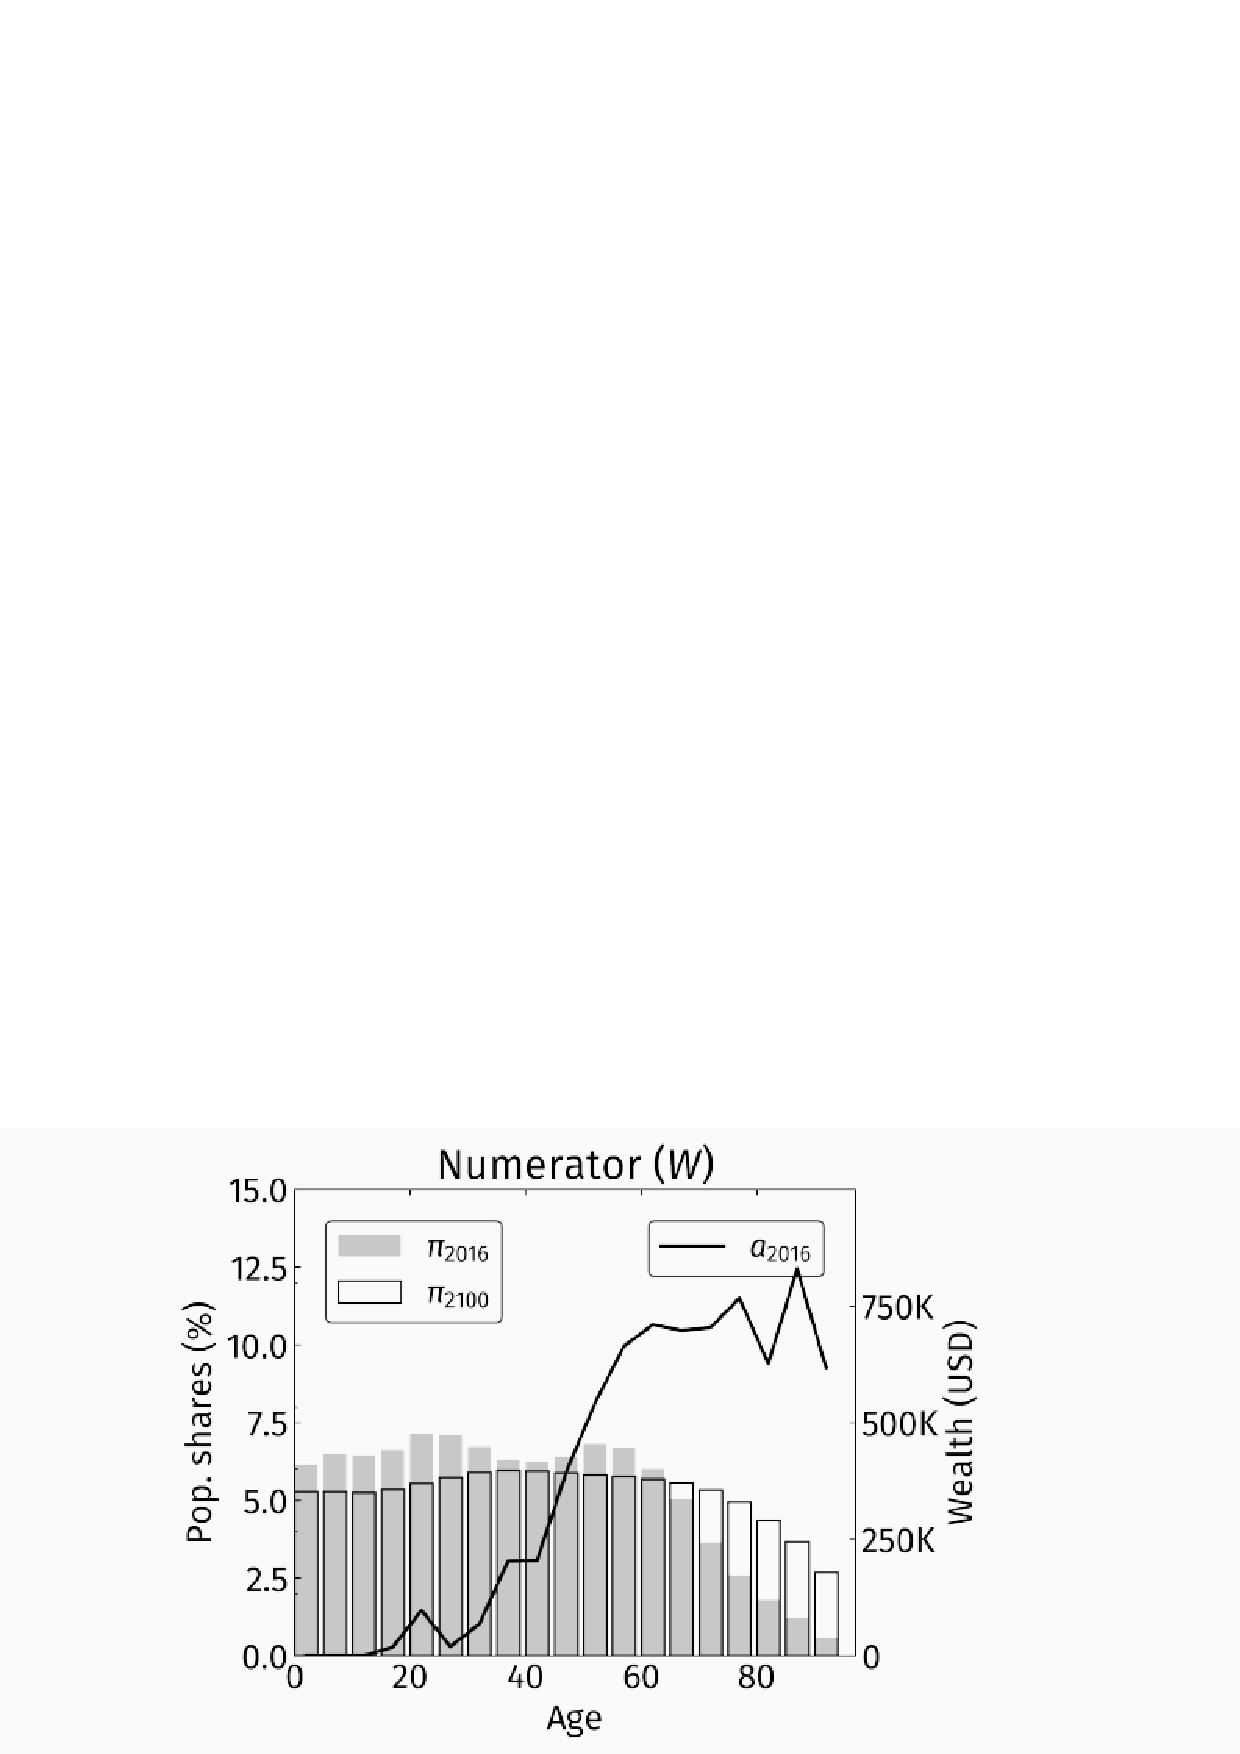
\includegraphics[width=0.9\paperwidth]{figs/Fig7b.PNG}
\par\end{center}

\end{frame}
%
\begin{frame}{Where do these large effects come from?}
\begin{itemize}
\item Does increase in W/Y come from increase in \textbf{wealth W}, or decrease
in \textbf{income Y}?
\end{itemize}
\begin{center}
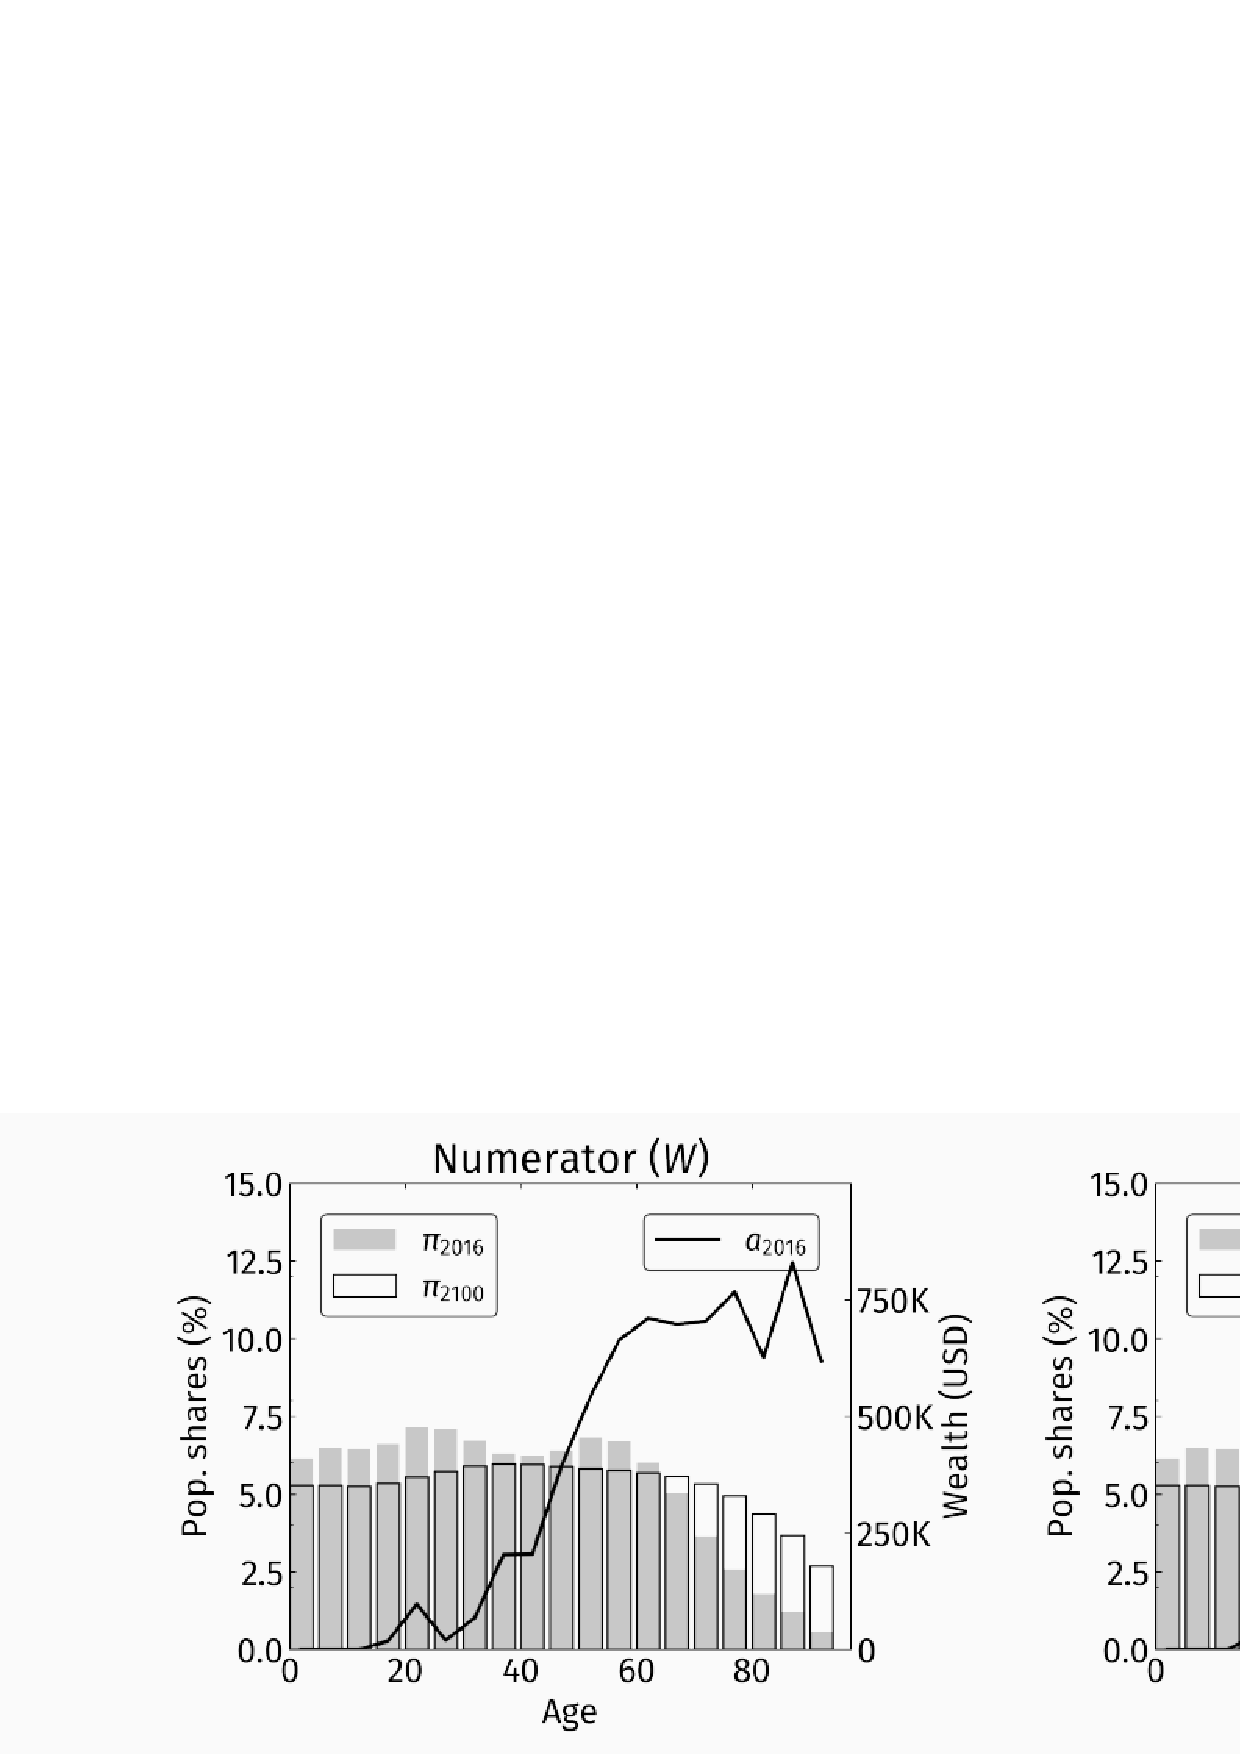
\includegraphics[width=0.9\paperwidth]{figs/Fig7c.PNG}
\par\end{center}

\end{frame}
%
\begin{frame}{Where do these large effects come from?}
\begin{center}
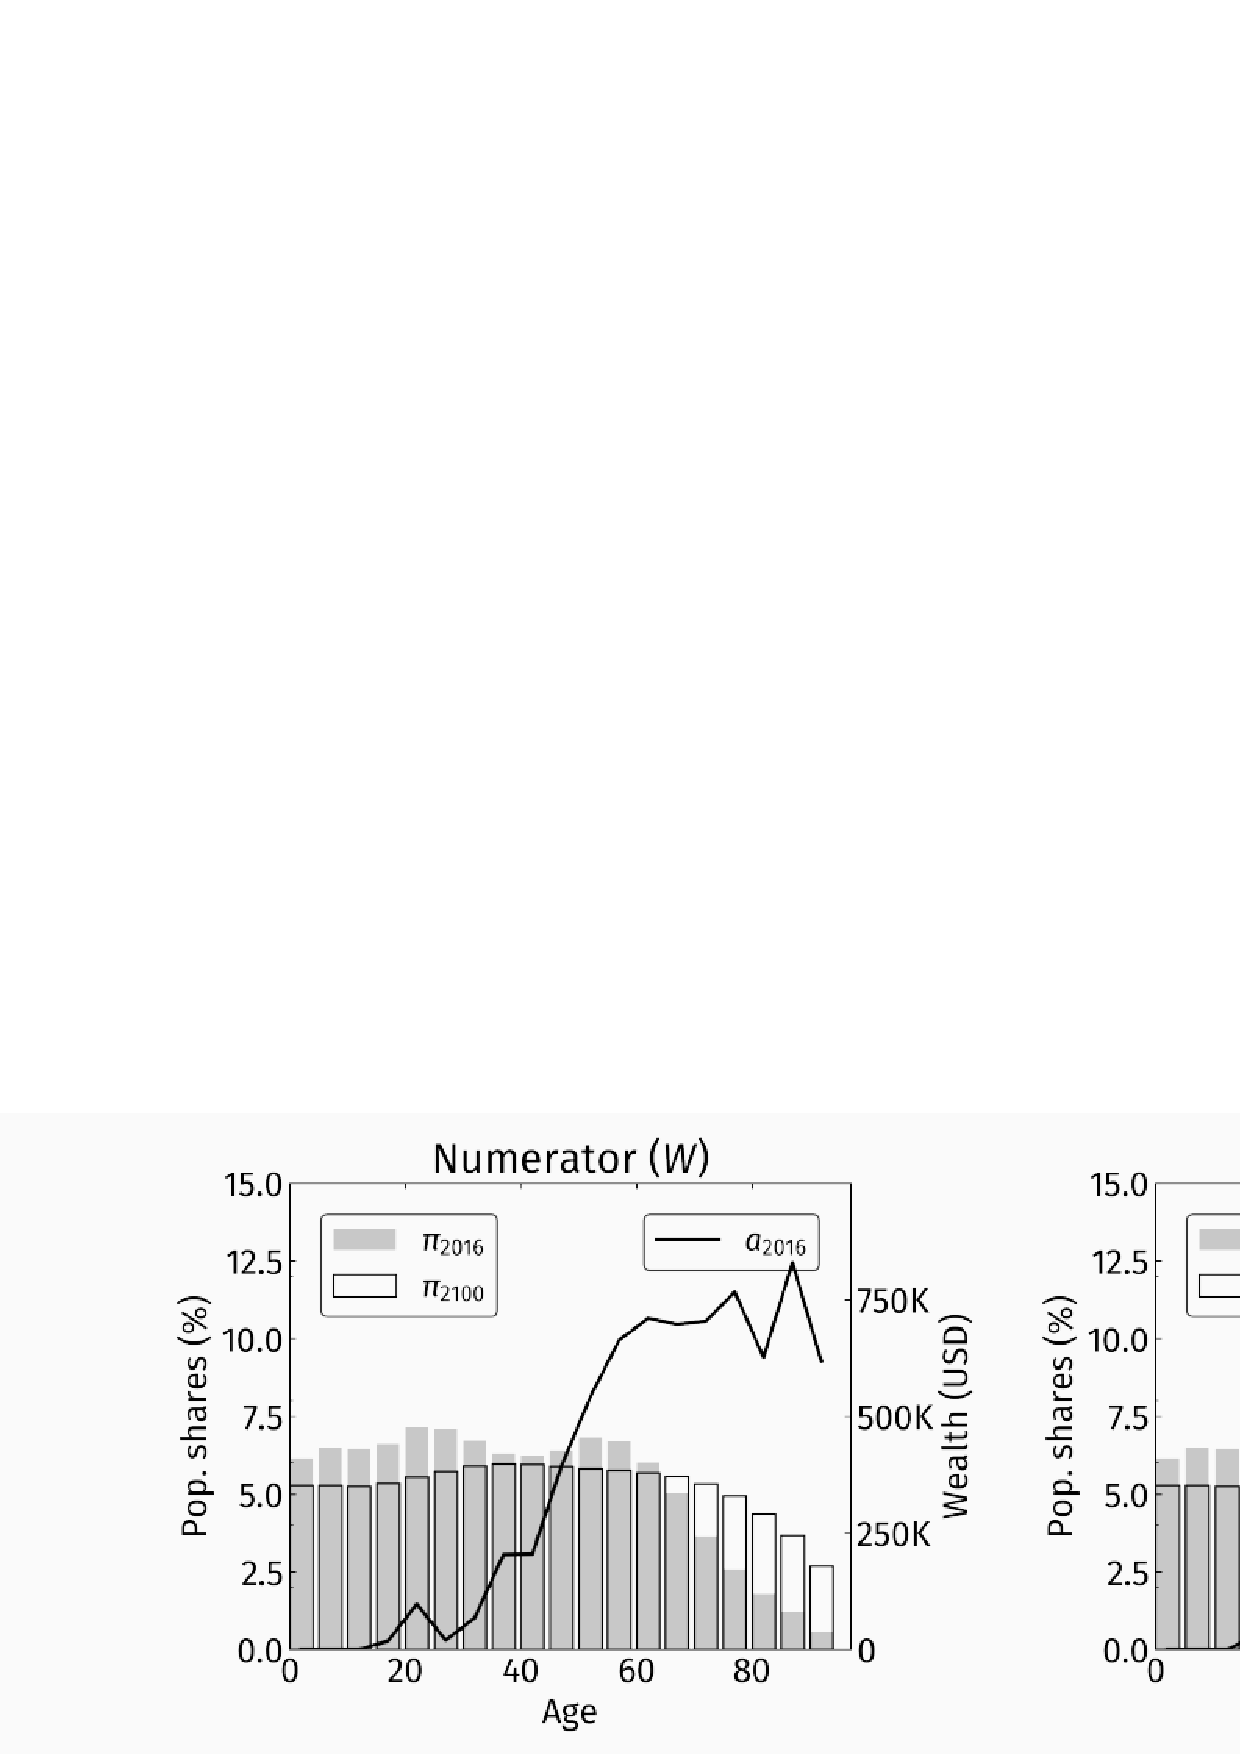
\includegraphics[width=0.9\paperwidth]{figs/Fig7c.PNG}
\par\end{center}
\begin{itemize}
\item In paper: separate contribution of numerator (wealth) and denominator
(income)
\begin{itemize}
\item Going forward: $W$ contributes $\sim2/3$, $Y$ contributes $\sim1/3$ 
\item Historically demographic dividend pushed $Y$ up, reversed in 2010
\end{itemize}
\end{itemize}
\end{frame}
%
\begin{frame}{Where do these large effects come from?}
\begin{center}
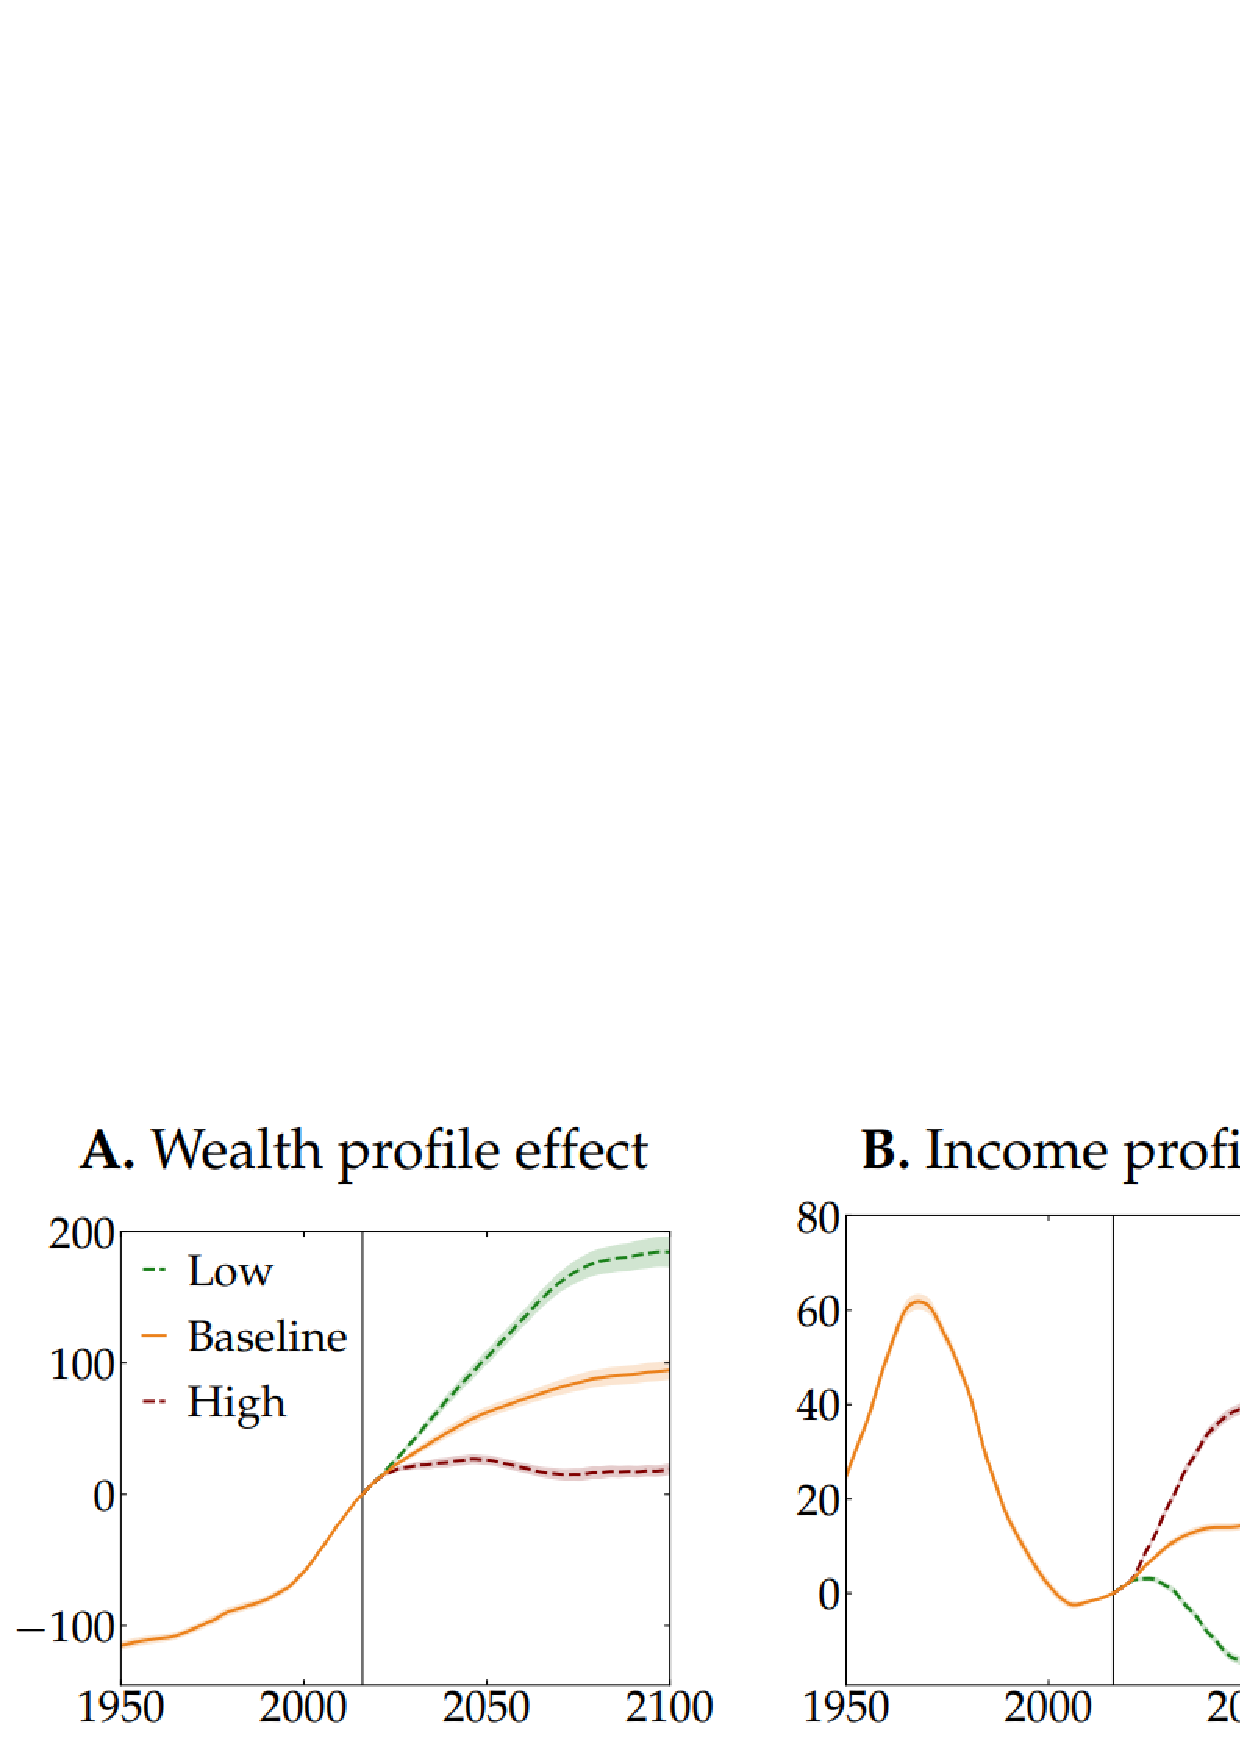
\includegraphics[width=0.9\paperwidth]{figs/Fig5-breakdown.PNG}
\par\end{center}
\begin{itemize}
\item <+->Historically (btw. 1970 and 2010) ``demographic dividend'' pushed
up $Y$, decreased $W/Y$ as a larger share of households were at
peak working age where labor income is highest
\item <+->But this effect has been less pronounced recently, as elderly
households earn less
\end{itemize}
\end{frame}
%
\begin{frame}{Across countries, $\Delta^{\text{comp }}$ large and heterogeneous
by 2100}

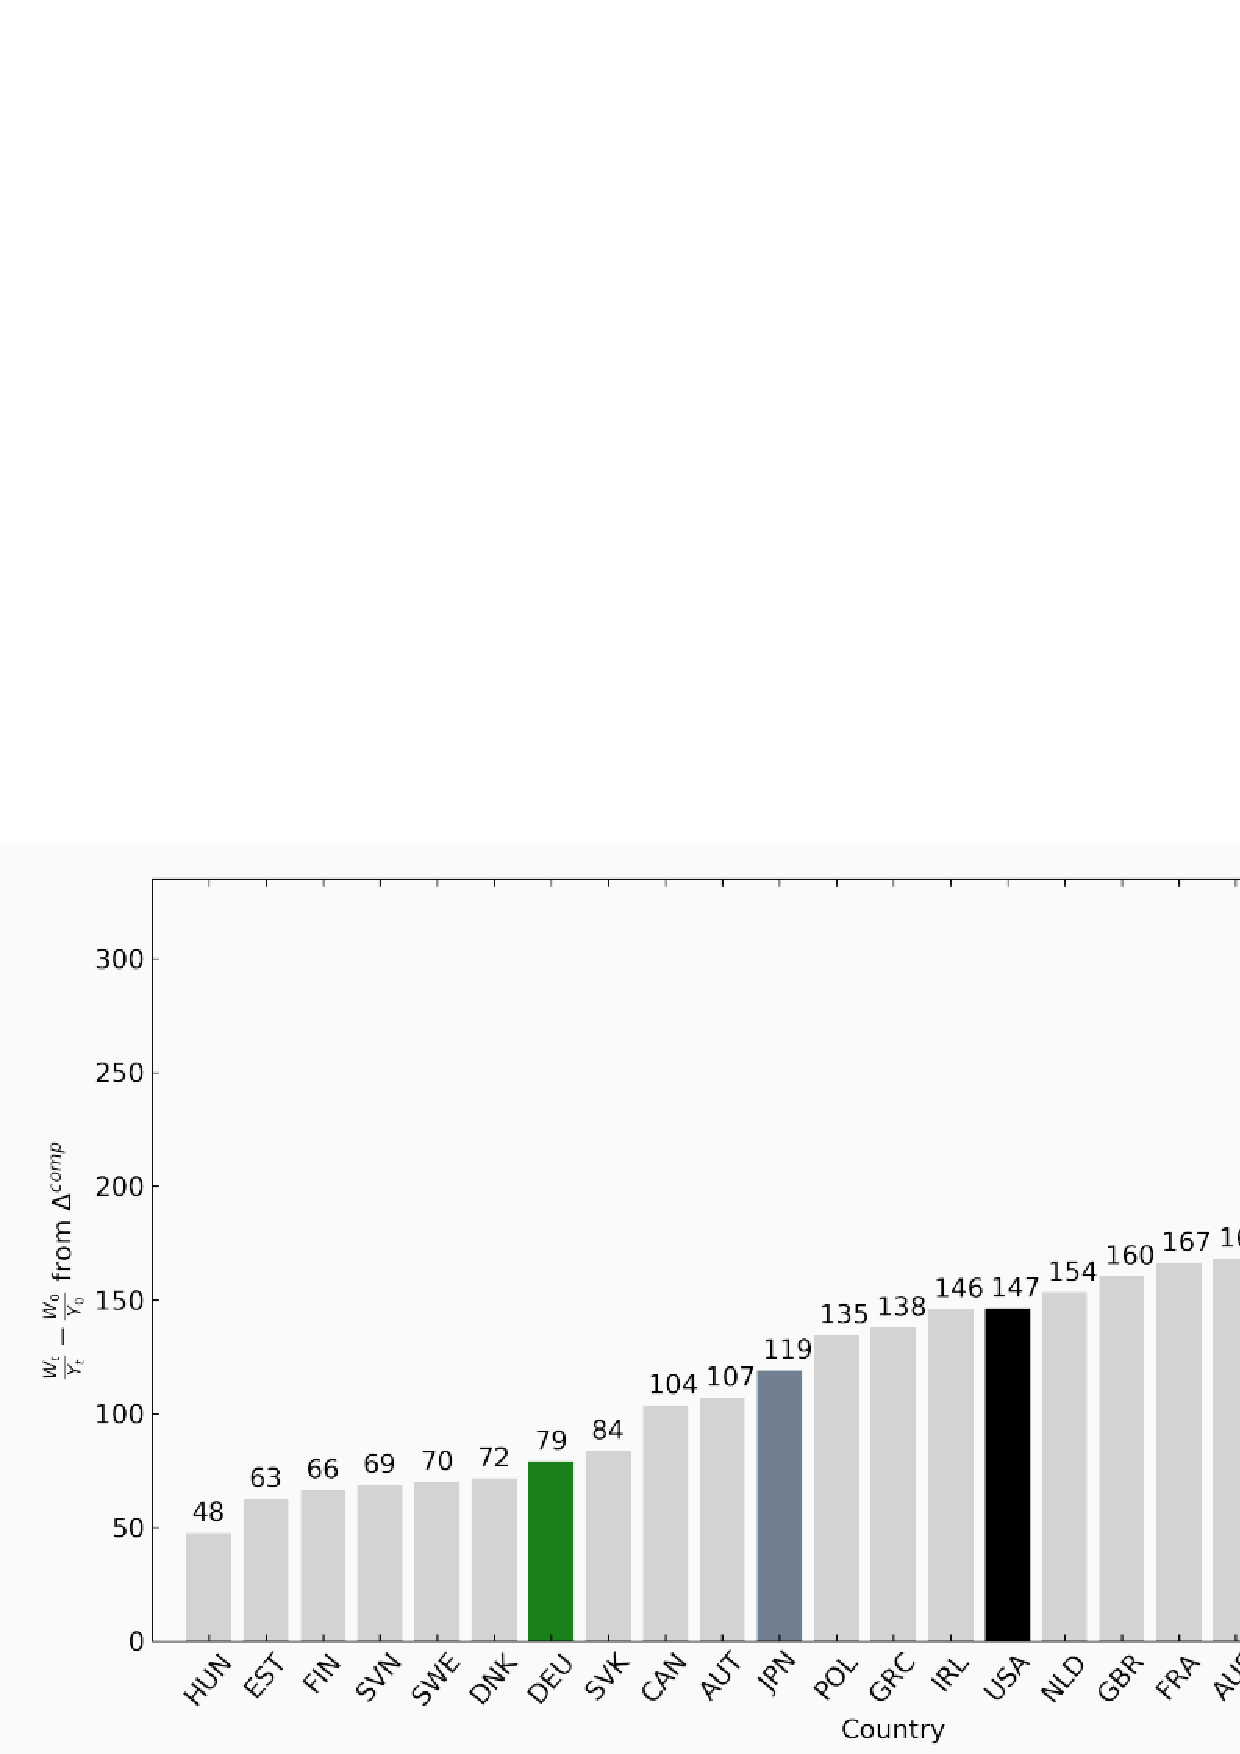
\includegraphics[width=0.8\paperwidth]{figs/Fig8.PNG}
\begin{itemize}
\item \textbf{Note}: Uses US saving/income age profiles
\end{itemize}
\end{frame}
%
\begin{frame}{General equilibrium }
\begin{itemize}
\item So far: Change age distribution keeping 
\begin{itemize}
\item World interest rate $r$ fixed 
\item Household consumption/saving behavior fixed 
\end{itemize}
\item Now: \textbf{General equilibrium}
\item Changing the age distribution will affect \emph{supply} of wealth
(demand for assets) 
\item Equilibrium $r$ will depend on supply of assets (gov. bonds + firm
capital) as well 
\end{itemize}
\end{frame}
%
\begin{frame}{General equilibrium implications}
\begin{center}
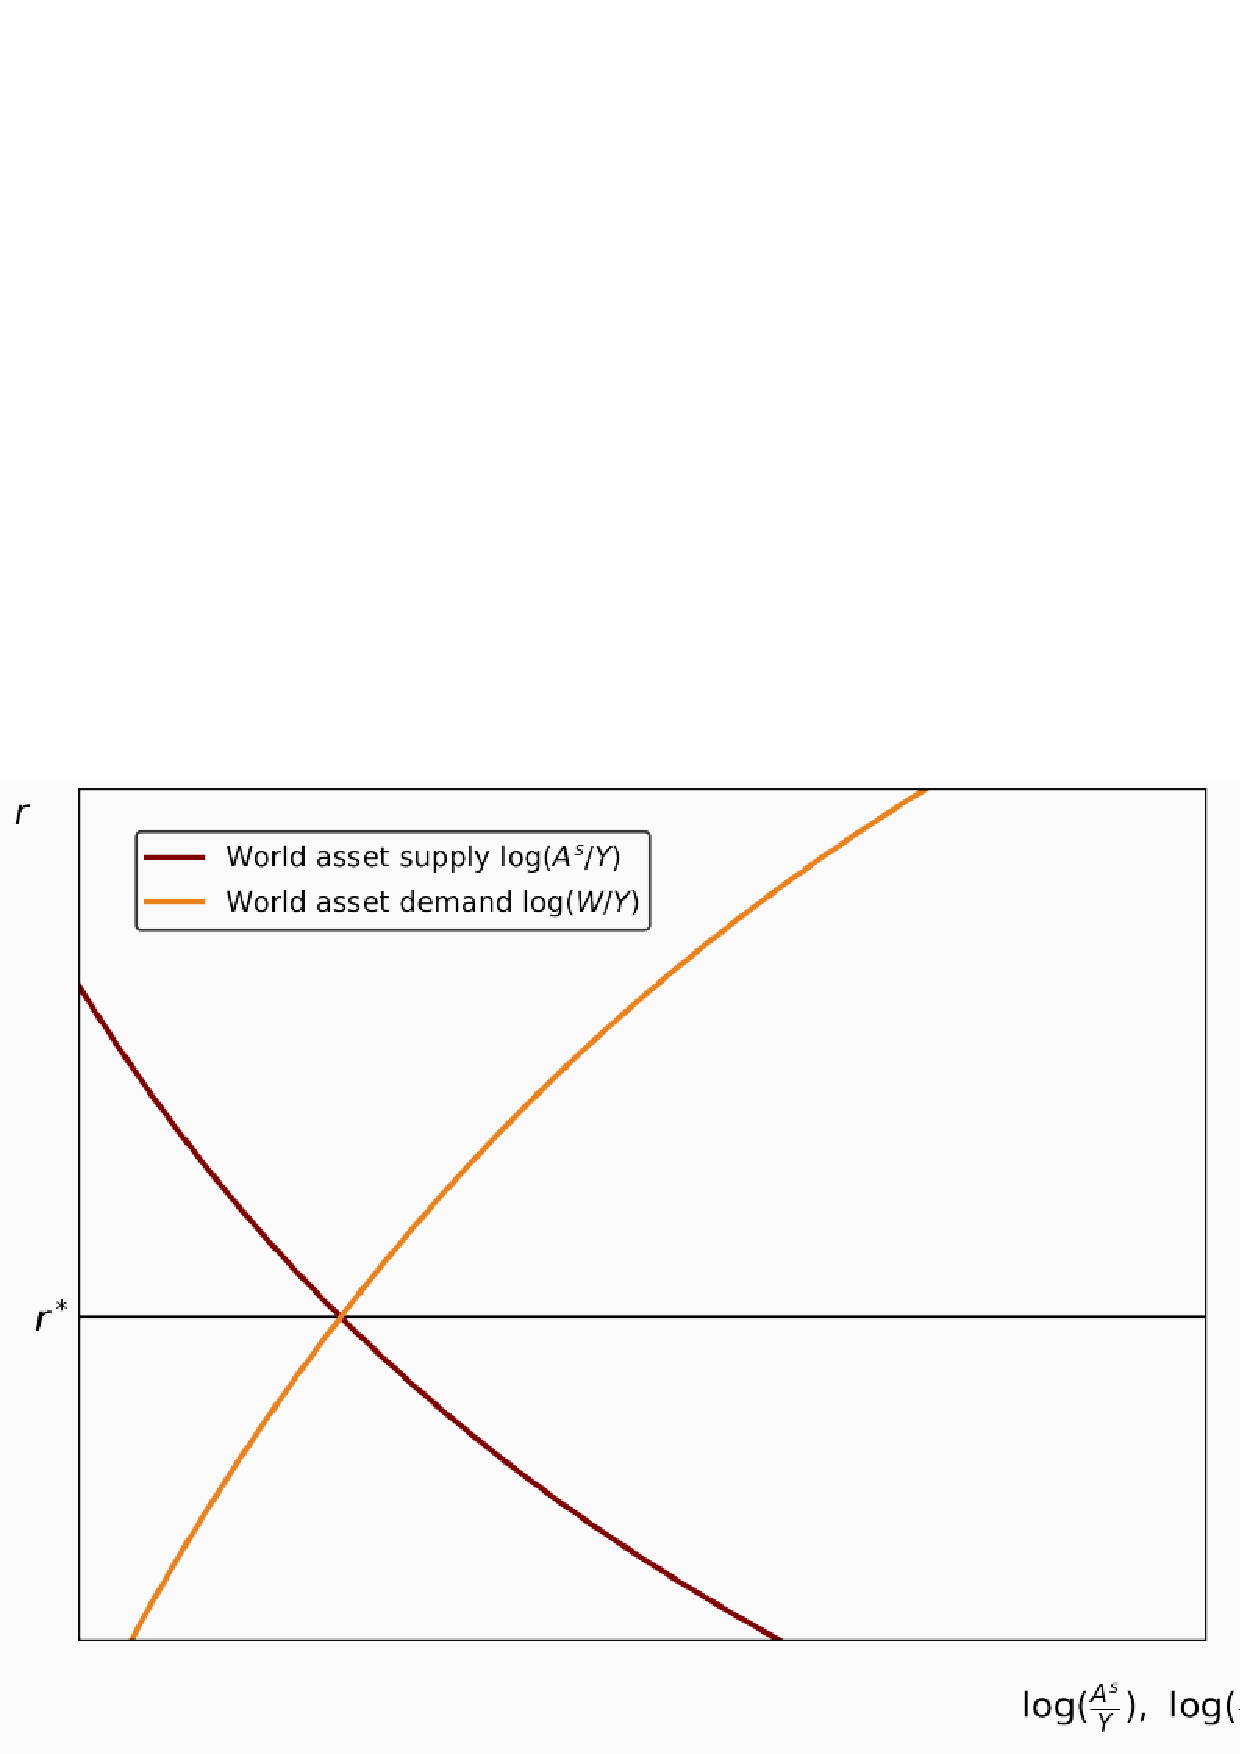
\includegraphics[width=0.6\paperwidth]{figs/Fig9a.PNG}
\par\end{center}

{\footnotesize Semielasticity of asset demand $\bar{\epsilon}_{d}=\frac{\partial\ln\left(W/Y\right)}{\partial r}$
: depends on elasticity of intertemporal substitution $\sigma$ and
observables (HHs)}{\footnotesize\par}

{\footnotesize Semielasticity of asset supply $\bar{\epsilon}_{s}=-\frac{\partial\ln\left((K+B)/Y\right)}{\partial r}$
: depends on elasticity of substitution between labor and capital}{\footnotesize\par}

{\footnotesize$\eta$ and observables (Firms + gov)}{\footnotesize\par}
\end{frame}
%
\begin{frame}{General equilibrium implications}
\begin{center}
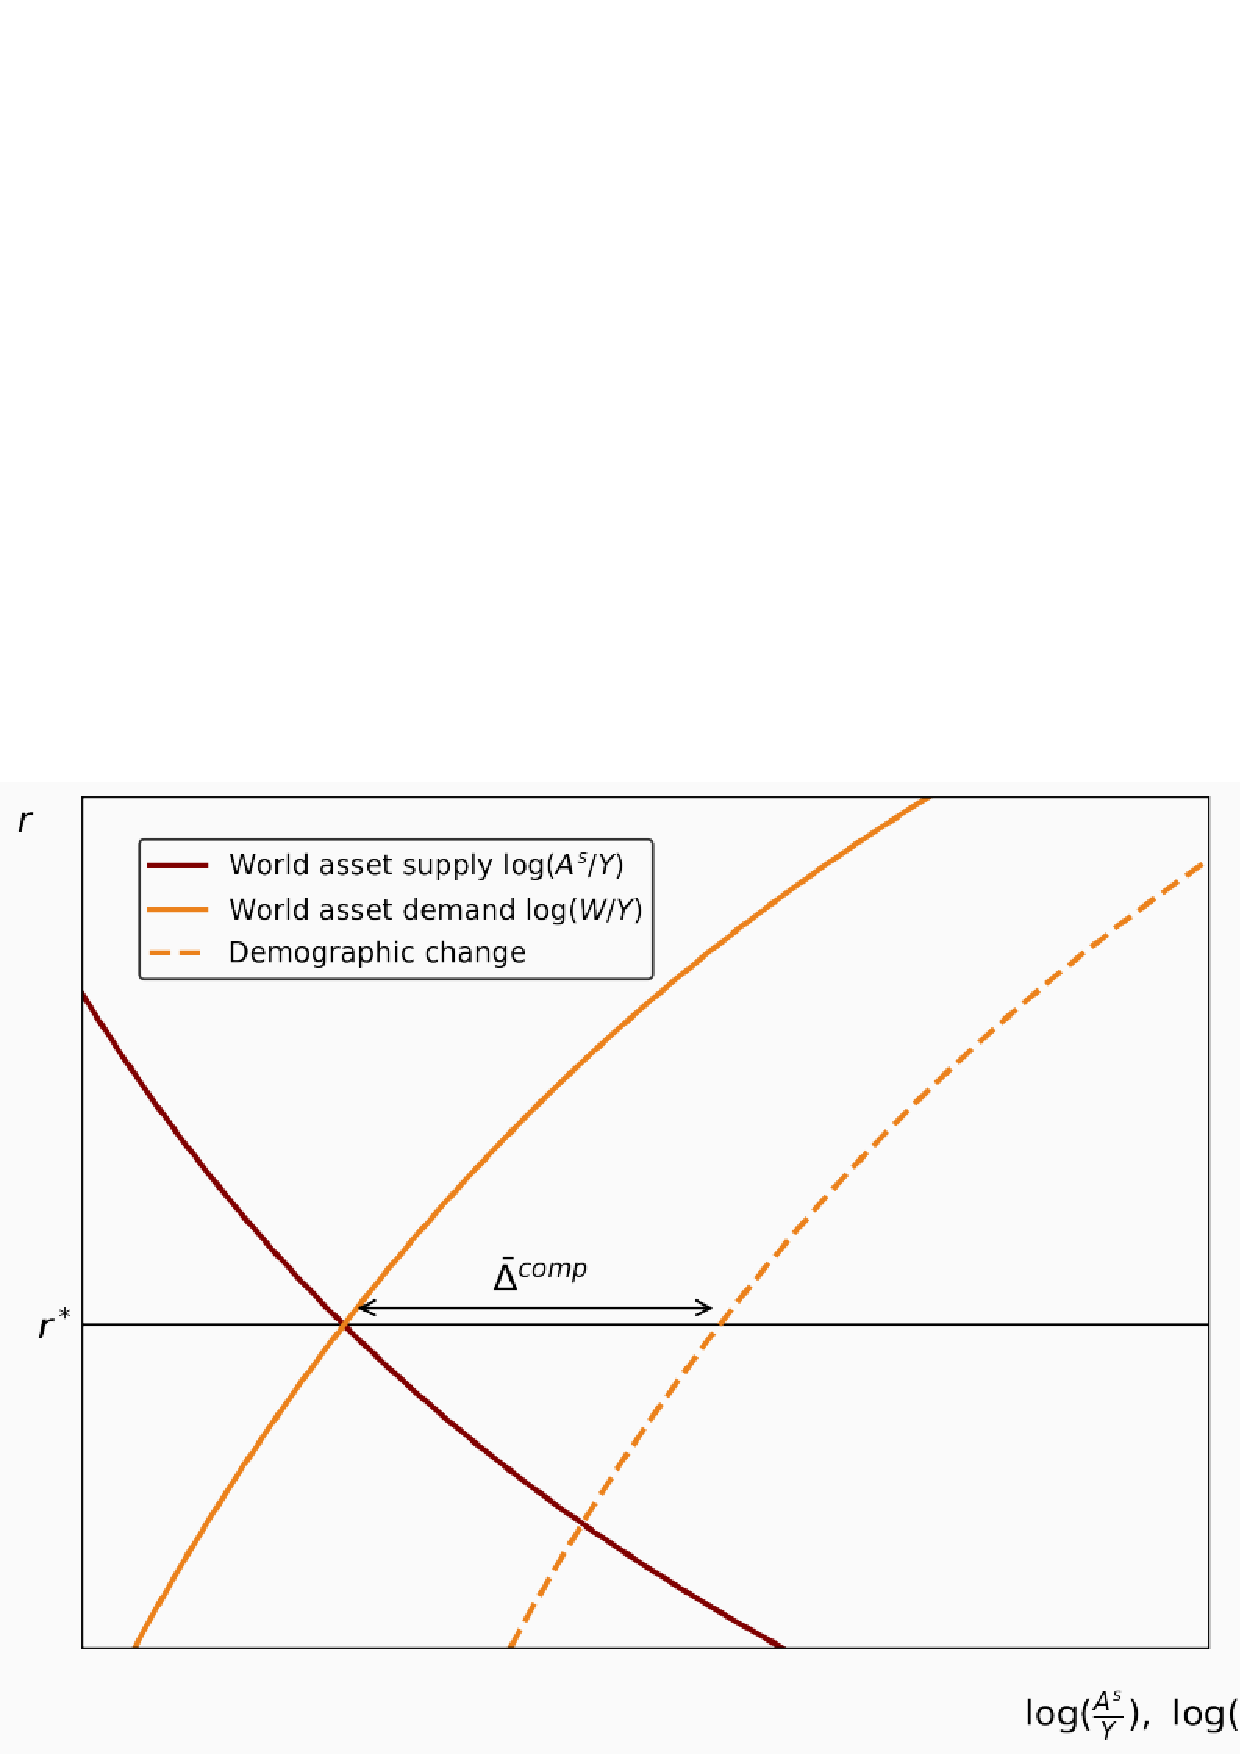
\includegraphics[width=0.6\paperwidth]{figs/Fig9b.PNG}
\par\end{center}

Asset demand shift of \textrm{$\overline{\Delta}^{\text{comp }}$}
: wealth-weighted average of $\Delta^{\text{comp, c }}$ 

Large and positive in the data.
\end{frame}
%
\begin{frame}{General equilibrium implications}
\begin{center}
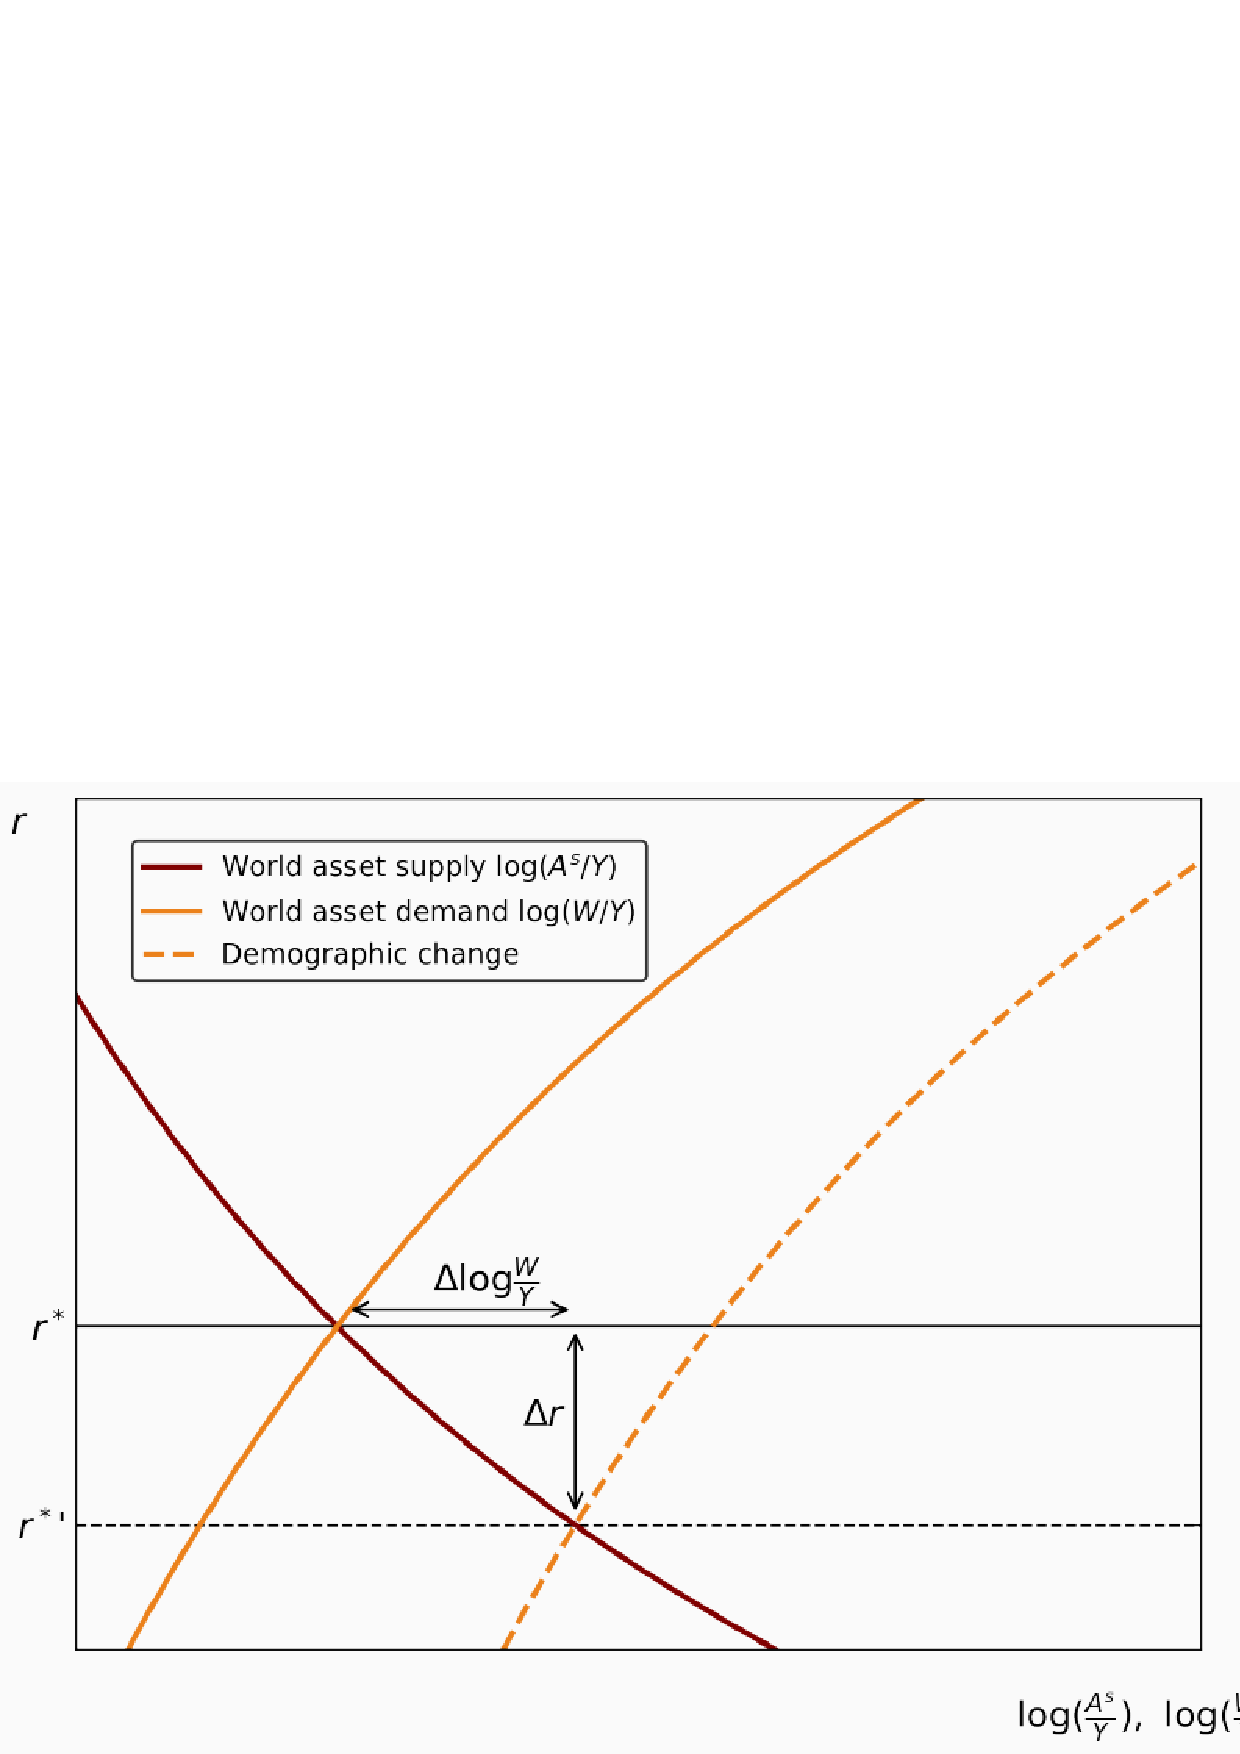
\includegraphics[width=0.6\paperwidth]{figs/Fig9c.PNG}
\par\end{center}

\end{frame}
%
\begin{frame}{General equilibrium implications}
\begin{block}{Proposition 2}

If the age profiles of assets and consumption are constant, net foreign
assets are zero, and governments maintain constaint debt-to-GDP ratios,
then the long run change in the rate of return is:
\[
\Delta r\approx-\frac{\bar{\Delta}^{\text{comp }}}{\bar{\epsilon}_{S}+\bar{\epsilon}_{d}}
\]
where $\bar{\epsilon}_{S}$ is the average semielasticity of asset
supply to $r,$and $\bar{\epsilon}_{d}$ is the average semielasticity
of asset holdings to $r$, and $\bar{\Delta}^{\text{comp }}$ is the
average compositional change. 

\end{block}
\begin{itemize}
\item If asset demand/capital supply is very elastic: Small decline in $r$
\begin{itemize}
\item HHs respond a lot to initial decline in $r$ by saving less (crowding
out direct effect $\bar{\Delta}^{\text{comp }}$), which stabilizes
$r$ in eq.
\item Firms respond by investing a lot in capital thereby driving up $r$
in eq.
\end{itemize}
\end{itemize}
\end{frame}
%
\begin{frame}{What determines the asset demand semielasticity?}

\[
\epsilon^{d}=\sigma\underbrace{\frac{C}{(1+g)W}\frac{\operatorname{Var}Age_{c}}{1+r}}_{\equiv\epsilon_{\text{substitution }}^{d}}+\underbrace{\frac{\mathbb{E}Age_{c}-\mathbb{E}Age_{a}}{1+r}}_{\equiv\epsilon_{\text{income }}^{d}}
\]

\begin{itemize}
\item <+->$Age_{a}$, $Age_{c}$: R.V. age weighted by assets/consumption
\item <+->The substitution effect: 
\begin{itemize}
\item Proportional to $\operatorname{Var}Age_{c}$ since there is more scope
for intertemporal substitution if consumption is more spread out over
the life cycle
\end{itemize}
\item <+->The income effect:
\begin{itemize}
\item Reflects the fact that a higher $r$ increases total income, if $\mathbb{E}Age_{a}<\mathbb{E}Age_{c}$
(i.e. the extra interest income is saved before it is consumed)
\item Note: Income effect can be negative since they allow for borrowing 
\end{itemize}
\item <+->The above can be measured assuming fixed $Age_{a}$ and $Age_{c}$ 
\begin{itemize}
\item The authors find $\epsilon_{\text{substitution }}^{d}=39.5$, $\epsilon_{\text{income }}^{d}=-2$,
thus $\epsilon^{d}>0$
\end{itemize}
\end{itemize}
\end{frame}
%
\begin{frame}{What determines the asset supply semielasticity?}

\[
\bar{\epsilon}^{s}=\frac{\eta}{r_{0}+\delta}\frac{\bar{K}_{0}}{\bar{W}_{0}}
\]

\begin{itemize}
\item <+->$\eta$ is the elasticity of substitution between capital and
labor
\item <+->$r_{0}+\delta=9.7\%$ is the user cost of capital
\item <+->$\frac{\bar{K}_{0}}{\bar{W}_{0}}=0.78$ is the initial global
capital-wealth ratio
\item <+->Based on the above calibration, $\bar{\epsilon}^{s}>0$ for any
plausible $\eta$.
\item <+-> Note: Holds for fixed gov. bond supply 
\end{itemize}
\end{frame}
%
\begin{frame}{Change in world interest rate}

Since $\bar{\epsilon}_{S}+\bar{\epsilon}_{d}>0$, then the change
in the world interest rate must be negative:
\[
\Delta r\approx-\frac{\bar{\Delta}^{\text{comp }}}{\bar{\epsilon}_{S}+\bar{\epsilon}_{d}}<0
\]
With different assumptions on the elasticity of intertemporal substitution
($\sigma$) and the elasticity of substitution between capital and
labor ($\eta$), this gives:
\[
\begin{tabular}{crrr}
  & \multicolumn{3}{c}{\ensuremath{\sigma} }\\
 \cline{ 2 - 4 } \ensuremath{\eta}  &  \ensuremath{0.25}  &  \ensuremath{0.50}  &  \ensuremath{1.00} \\
\hline  \ensuremath{0.60}  &  \ensuremath{-3.24}  &  \ensuremath{-1.59}  &  \ensuremath{-0.79} \\
 \ensuremath{1.00}  &  \ensuremath{-2.09}  &  \ensuremath{-1.25}  &  \ensuremath{-0.70} \\
 \ensuremath{1.25}  &  \ensuremath{-1.71}  &  \ensuremath{-1.10}  &  \ensuremath{-0.65} \\
\hline  
\end{tabular}
\]

\end{frame}
%
\begin{frame}{Change in capital to income ratio}

Proposition 2 gives a similar formula for the change in capital to
income:
\[
\overline{\Delta\log\left(\frac{W}{Y}\right)}\approx\frac{\bar{\epsilon}_{\mathrm{S}}}{\bar{\epsilon}_{\mathrm{S}}+\bar{\epsilon}_{d}}\bar{\Delta}^{\text{comp }}>0
\]

Again with different assumptions on the IES ($\sigma$) and the elasticity
of substitution between capital and labor ($\eta$)
\[
\begin{tabular}{cccc}
  & \multicolumn{3}{c}{\ensuremath{\sigma} }\\
 \cline{ 2 - 4 } \ensuremath{\eta}  &  \ensuremath{0.25}  &  \ensuremath{0.50}  &  \ensuremath{1.00} \\
\hline  \ensuremath{0.60}  &  \ensuremath{15.6}  &  \ensuremath{7.7}  &  \ensuremath{3.8} \\
 \ensuremath{1.00}  &  \ensuremath{16.7}  &  \ensuremath{10.0}  &  \ensuremath{5.6} \\
 \ensuremath{1.25}  &  \ensuremath{17.1}  &  \ensuremath{11.1}  &  \ensuremath{6.5} \\
\hline  
\end{tabular}
\]

The authors argue that simulations from the general model deliver
similar outcomes
\end{frame}
%
\begin{frame}{Change in net foreign assets}
\begin{center}
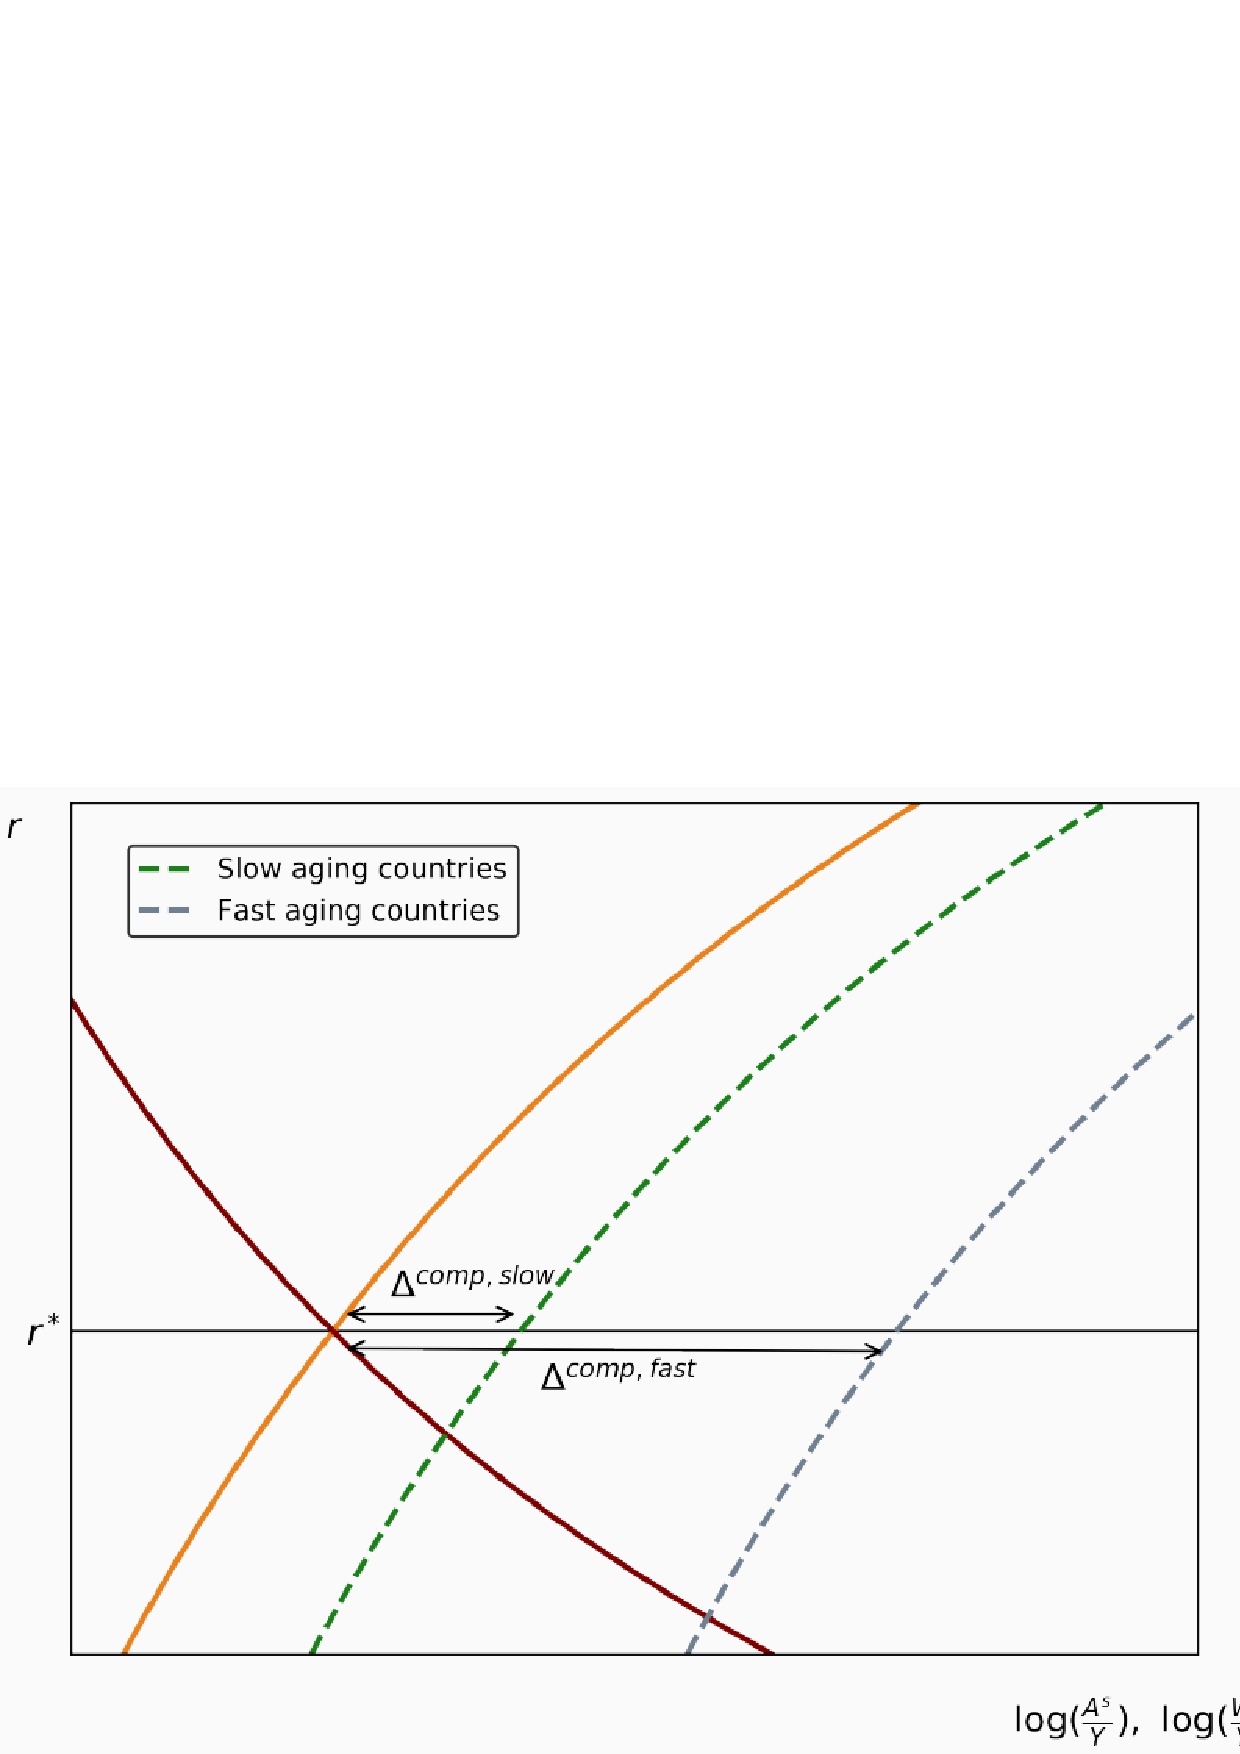
\includegraphics[width=0.6\paperwidth]{figs/Fig9d.PNG}
\par\end{center}

Country specific $\Delta^{\text{comp}}$ large and heterogeneous in
the data 
\end{frame}
%
\begin{frame}{Change in net foreign assets}
\begin{center}
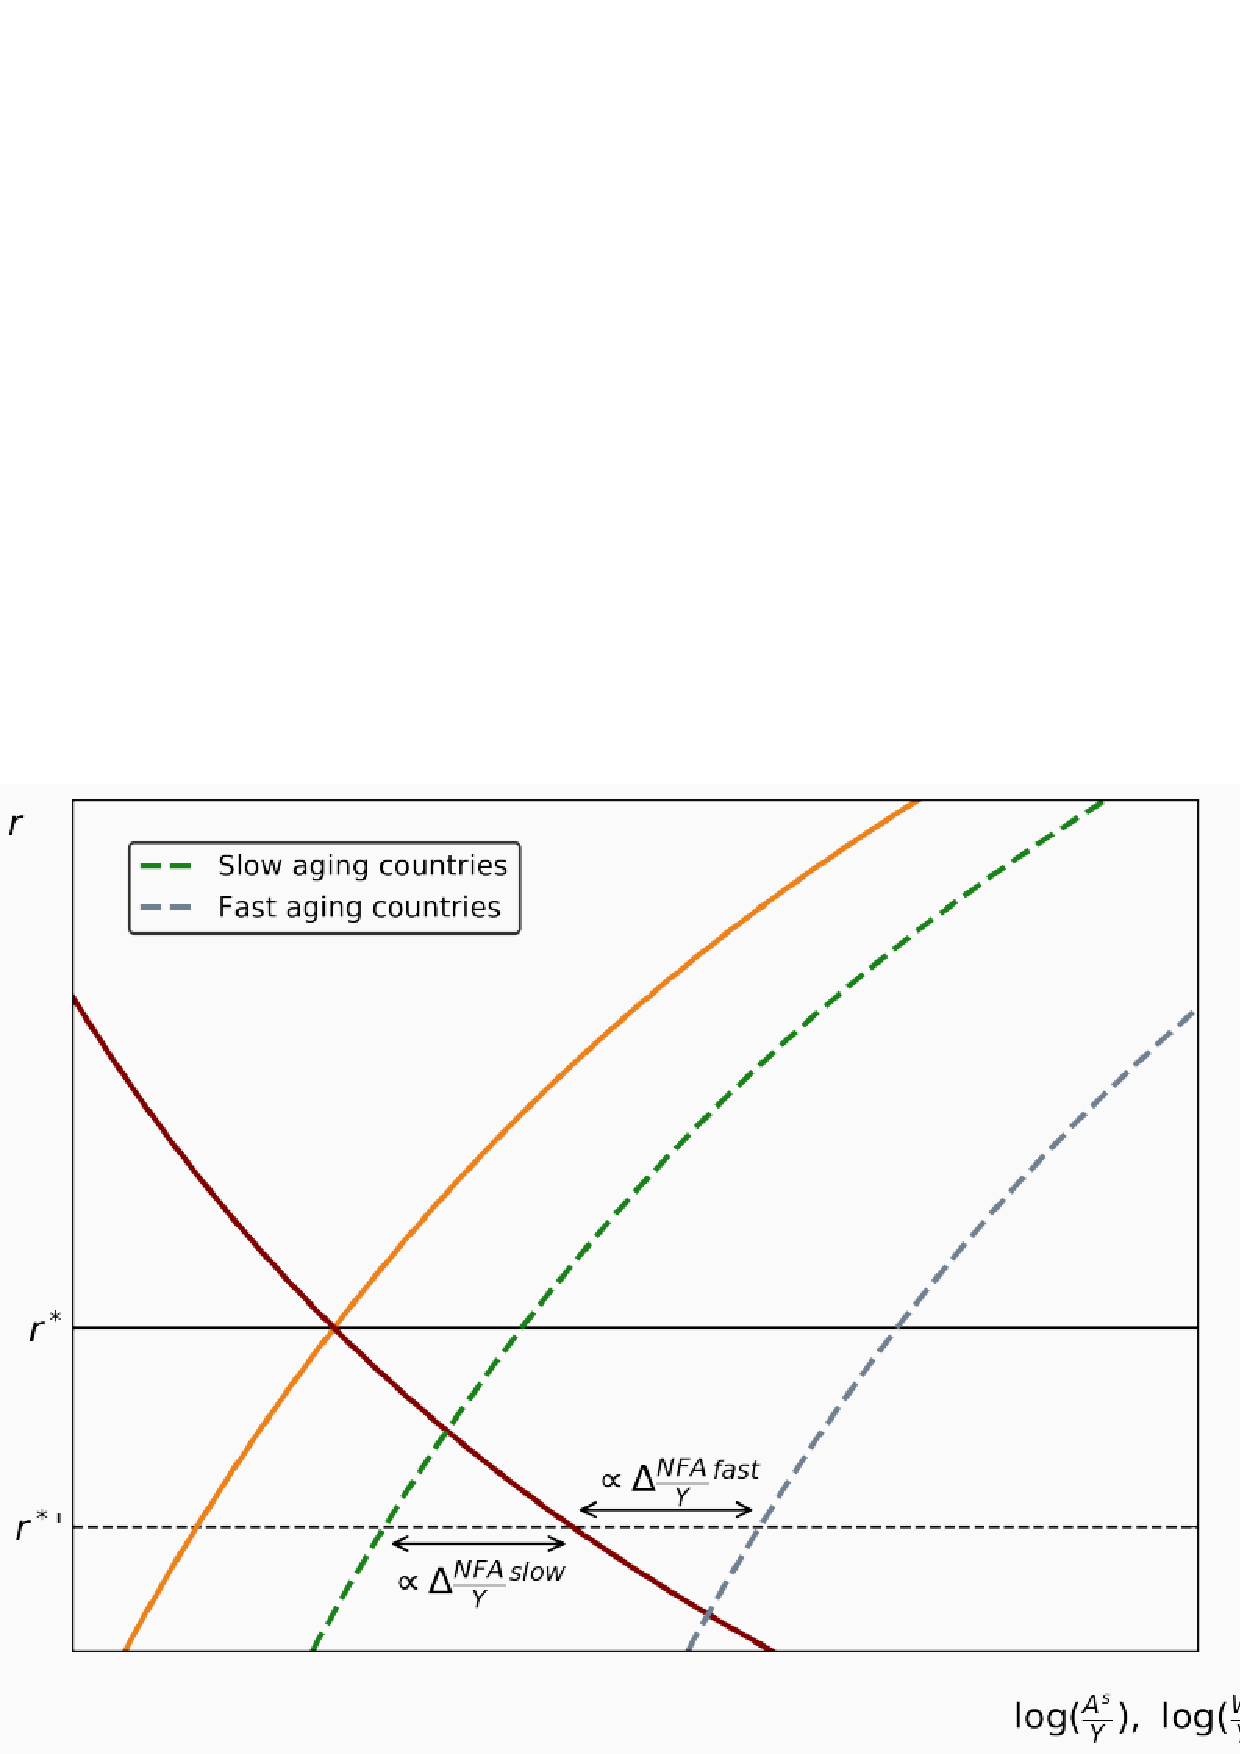
\includegraphics[width=0.4\paperwidth]{figs/Fig9e.PNG}
\par\end{center}
\begin{itemize}
\item <+->Countries that age faster will accumulate more wealth, which
it supplies to the rest of the world (NFA>0)
\begin{itemize}
\item Particularly to countries that age slowly (less wealth accumulation)
where domestic firms need to go abroad for investments
\end{itemize}
\end{itemize}
\[
\Delta\left(\frac{NFA}{Y}\right)\approx\frac{W_{0}}{Y_{0}}\left(\Delta^{\text{comp,c }}-\bar{\Delta}^{\text{comp }}\right)
\]

\end{frame}
%
\begin{frame}{Change in net foreign assets}
\begin{center}
\[
\Delta\left(\frac{NFA}{Y}\right)\approx\frac{W_{0}}{Y_{0}}\left(\Delta^{\text{comp,c }}-\bar{\Delta}^{\text{comp }}\right)
\]
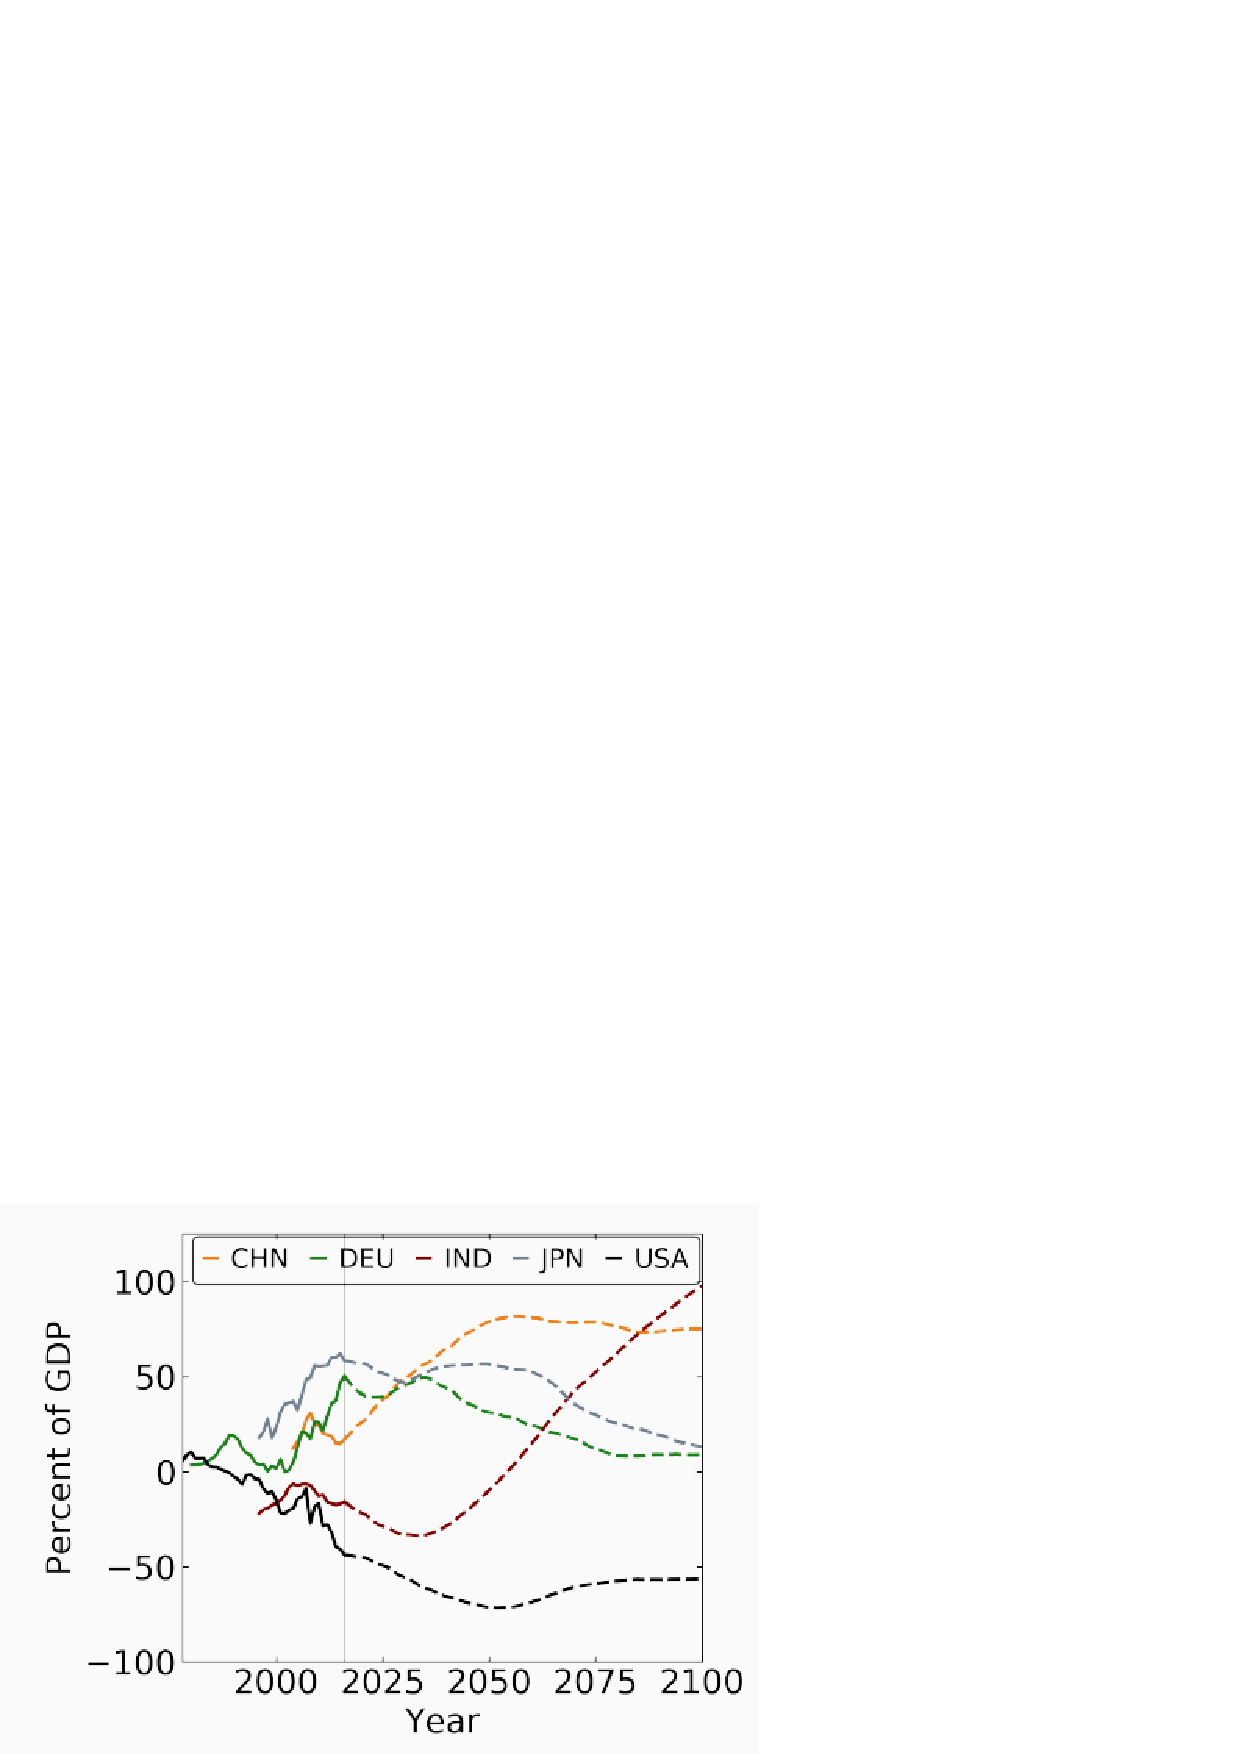
\includegraphics[width=0.5\paperwidth]{figs/Fig10.PNG}
\par\end{center}

$\rightarrow$ Data suggest large global imbalances going forward
\end{frame}
%
\begin{frame}{Limitation to baseline model}
\begin{itemize}
\item <+->What are some limitations of their baseline analysis?
\begin{itemize}
\item <+->Demographics have no effect on individual savings
\item <+->Demographics have no effect on the tax-and-transfer system
\item <+->No bequest motives
\item <+->No changes in mortality (only birth rates)
\item <+->Demographics have no effect on TFP growth
\end{itemize}
\item <+->To study some of these changes, the authors extend their baseline
model $\rightarrow$ then simulate the transition path 
\end{itemize}
\end{frame}
%
\begin{frame}{Results from richer model}
\begin{itemize}
\item <+->Compositional effect by country from analytical model product
of:
\begin{itemize}
\item Combination of demographic changes (exogenous in model) and labor
supply/wealth profiles (endogenous)
\end{itemize}
\item <+->Could match perfectly in richer model if model could replicate
observed wealth and labor profiles over the lifecycle 
\item <+->Main finding: $\Delta^{comp}$ in the richer model is roughly
similar to the results from the data
\end{itemize}
\end{frame}
%
\begin{frame}{Results from richer model}
\begin{itemize}
\item Compositional effect by country from analytical model product of:
\begin{itemize}
\item Combination of demographic changes (exogenous in model) and labor
supply/wealth profiles (endogenous)
\end{itemize}
\item Could match perfectly in richer model if model could replicate observed
wealth and labor profiles over the lifecycle 
\item Main finding: $\Delta^{comp}$ in the richer model is roughly similar
to the results from the data
\end{itemize}
\begin{center}
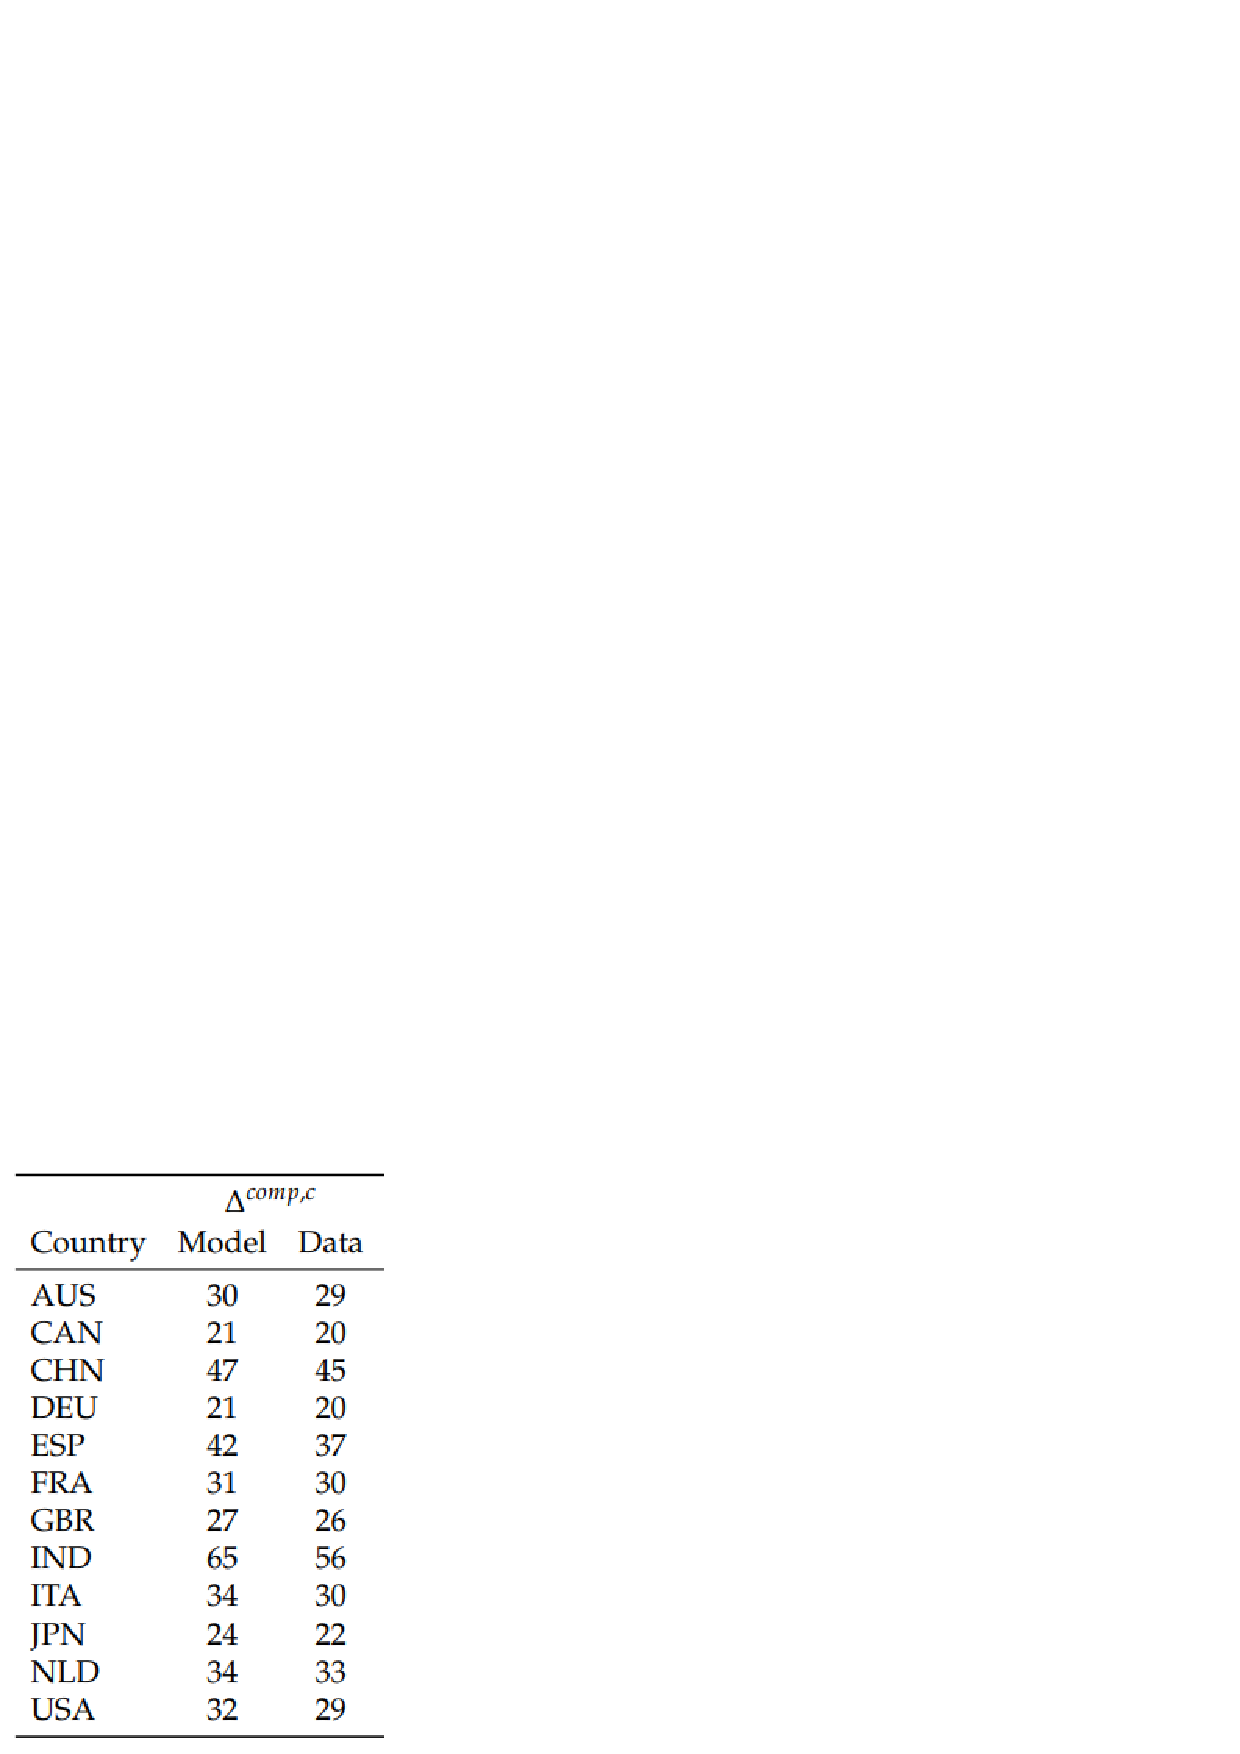
\includegraphics[width=0.2\paperwidth]{figs/Table1.PNG}
\par\end{center}

\end{frame}
%
\begin{frame}{Results from richer model}
\begin{itemize}
\item GE Effects from the model are also roughly similar

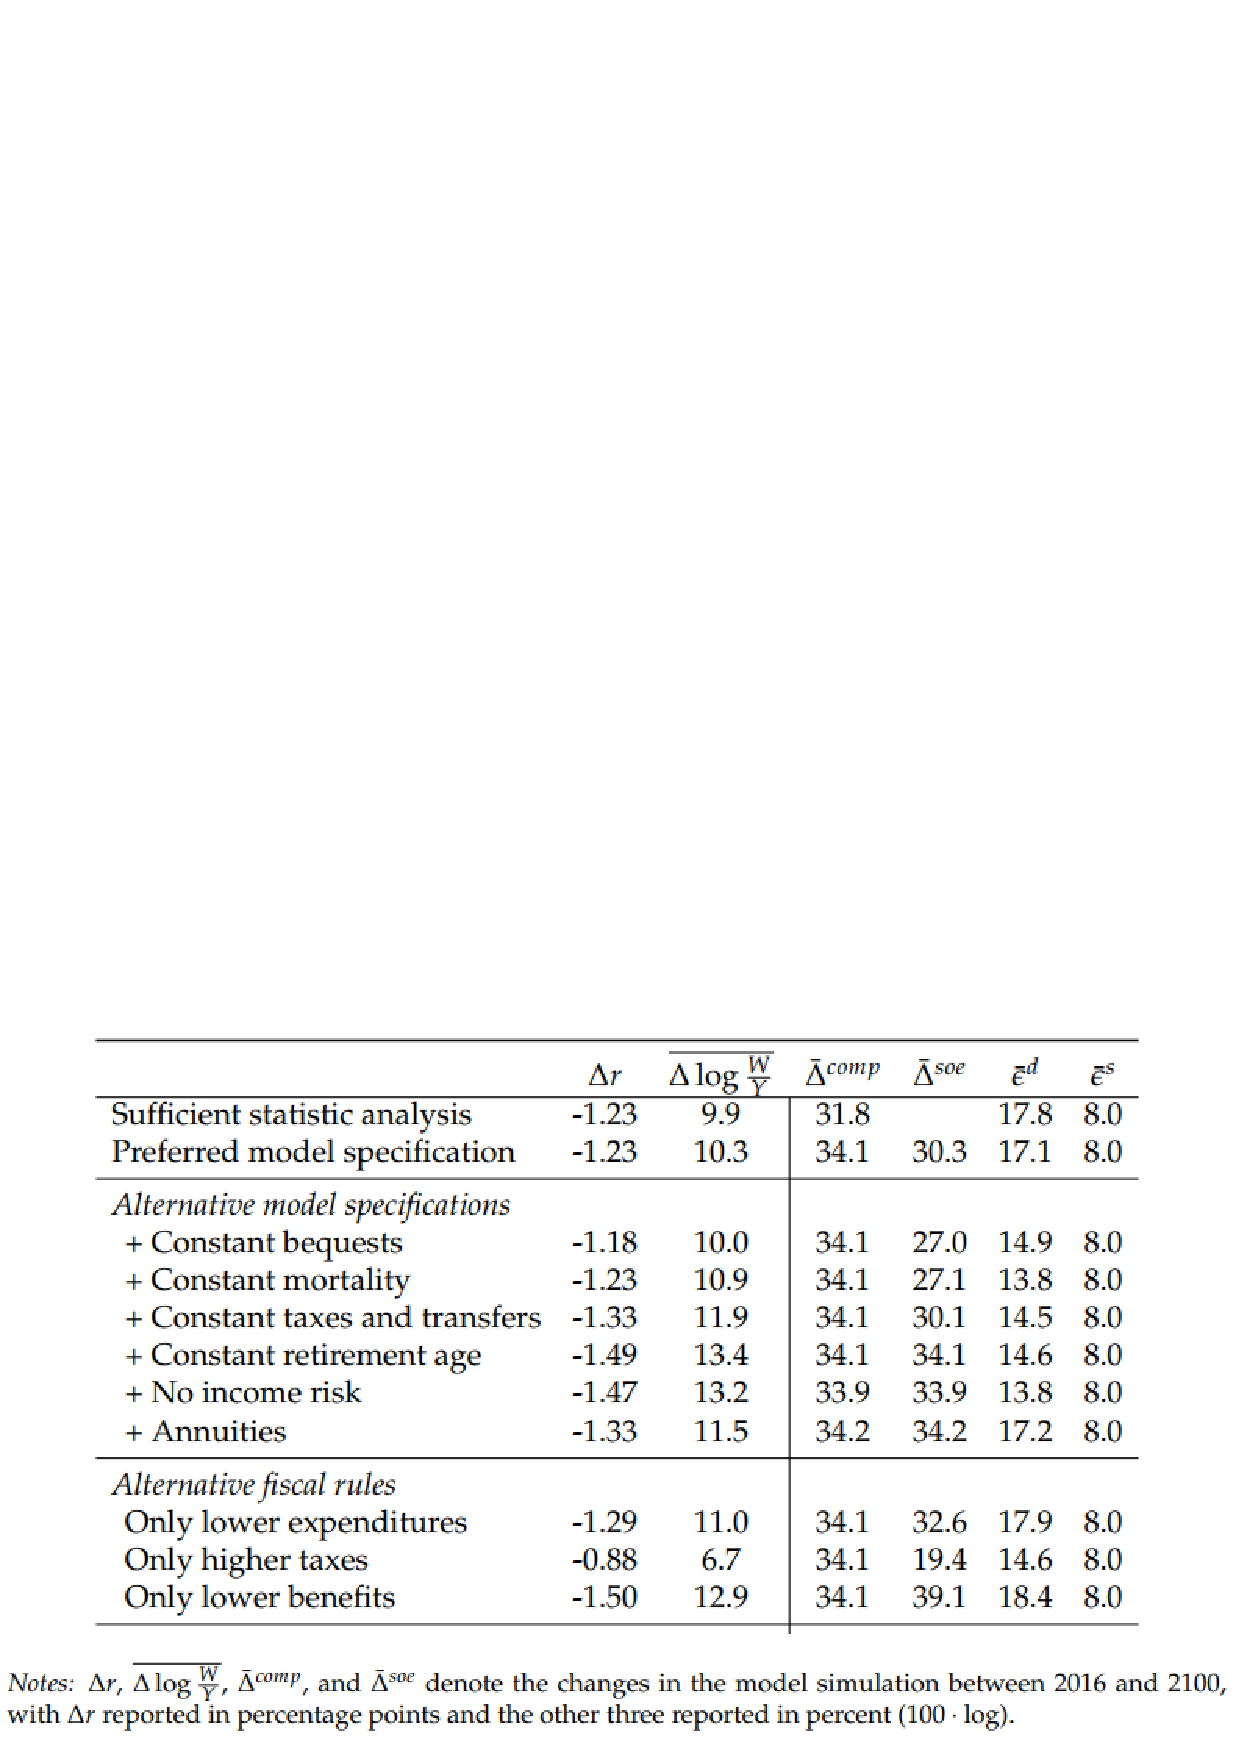
\includegraphics[width=0.8\paperwidth]{figs/Table2.PNG}
\end{itemize}
\end{frame}
%
\begin{frame}{Conclusion}
\begin{itemize}
\item <+->How does population aging affect wealth-output ratios, real interest
rates, and capital flows?
\begin{itemize}
\item what matters is the compositional effect $\Delta^{\text{comp }}$
\item large and heterogeneous in the data
\end{itemize}
\item <+->The approach developed by the authors:
\begin{itemize}
\item Refutes the asset market meltdown hypothesis: $r$ falls 
\item Suggests wealth-to-income ratio will keep rising 
\item Larger global imbalances (dispersion of NFAs)
\end{itemize}
\end{itemize}
\end{frame}
%

\section{Income Inequality \\ Straub (2019)}
\begin{frame}{Secular stagnation and income inequality}
\begin{itemize}
\item <+->Auclert et al (2021) explains decline in $r$ and rise in $\frac{W}{Y}$
with demographic shifts 
\item <+->Parallel literature explains decline through \emph{rising} income/wealth
\textbf{inequality }
\begin{itemize}
\item See i.e. Mian, Sufi, Straub (2021): \emph{What explains the decline
in r{*}? Rising income inequality versus demographic shifts}
\end{itemize}
\item <+->\textbf{Example}: If saving rates increase with income (richer
save more) then:
\begin{itemize}
\item Redistribution from poor to rich households \emph{increase} the aggregate
supply of savings $\Rightarrow$ lower rates in GE
\item Suggests link between increasing income inequality and secular stagnation 
\item Straub (2019, WP) tests this hypothesis 
\end{itemize}
\end{itemize}
\end{frame}


\begin{frame}{Stylized model}

\begin{itemize}
  \item Deterministic model with one-period lived households \pause
  \item Constant wage $w$, return $R$ \pause
  \item Get utility from consumption $c_t$ and wealth $a_{t+1}$ \pause 
\end{itemize}
$$\begin{aligned}
\max_{c_t,a_{t+1}} u(c_t)+\beta U(a_{t+1}) \\
c_t +R^{-1} a_{t+1}\leq a_t + w_t   
\end{aligned}$$
with $u(c)=\frac{c^{1-\sigma}}{1-\sigma}$ and $U(a)=\frac{a^{1-\Sigma}}{1-\Sigma}$ \\ \pause
We can show that $c_t \approx k(a_t+w)^\phi$, with $\phi=\frac{\Sigma}{\sigma}$
\end{frame}


%
\begin{frame}{Empirical estimate}
\begin{itemize}
\item <+->We can check in the data the empirical relationship between permanent income and consumption
\item <+->If $\phi<1$ consumption rises \emph{less} than proportionally
with income
\begin{itemize}
\item I.e. savings rise \emph{more $\Rightarrow$ }Richer HHs save more 
\item Opposite for $\phi>1$
\end{itemize}
\item <+->Two questions
\begin{itemize}
\item What does this elasticity look like emprically?
\item If $\phi\neq1$ how can we accomodate this in a HA model?
\end{itemize}
\end{itemize}
\end{frame}


\begin{frame}{Empirical estimate}
\begin{itemize}
\item <+->Use US panel survey data (PSID)
\item <+->Regress $\log c_{it}$ on controls (year, age, HH size, location)
and 9 year average of income
\item <+->Binned scatter:\\
\begin{figure}[H]     
\centering      
\includegraphics[width=0.5\linewidth]{figs/Straub2019Scatter.PNG}      
\end{figure}
\item <+->More detalied estimates in paper, suggest $\phi\approx0.7$
\end{itemize}
\end{frame}


\begin{frame}{Permanent redistribution in the canonical HA model}
\begin{itemize}

\item <+->Consider standard HA model with permanent income state $p:$
\[
\begin{aligned}V\left(a_{t-1},z_{t},p\right)= & \max_{c_{t}}\frac{c_{t}^{1-\sigma}}{1-\sigma}+\beta\mathbb{E}\left[V\left(a_{t},z_{t+1},p\right)\right]\\
 & \text{ subject to }\\
 & c_{t}+a_{t}=Ra_{t-1}+z_{t}p\\
 & a_{t}\geq0\\
\ln z_{t} & =\rho\ln z_{t-1}+\epsilon_{t}
\end{aligned}
\]
\item <+->Note: preferences are \emph{homothetic }(homogeneous of degree
1)
\begin{itemize}
\item >>Scale independent<<
\end{itemize}
\end{itemize}
\end{frame}

%
\begin{frame}{Homothetic household problem I}
\begin{itemize}
\item <+->Normalize constraints by $p$ and Bellman by $p^{1-\sigma}$
\[
\begin{aligned}\frac{V\left(a_{t-1},z_{t},p\right)}{p^{1-\sigma}}= & \max_{c_{t}}\frac{\frac{c_{t}^{1-\sigma}}{1-\sigma}}{p^{1-\sigma}}+\beta\frac{\mathbb{E}\left[V\left(a_{t},z_{t+1},p\right)\right]}{p^{1-\sigma}}\\
 & \text{ subject to }\\
 & \frac{c_{t}}{p}+\frac{a_{t}}{p}=R\frac{a_{t-1}}{p}+z_{t}\frac{p}{p}\\
 & \frac{a_{t}}{p}\geq\frac{0}{p}
\end{aligned}
\]
\end{itemize}
\end{frame}
%
\begin{frame}{Homothetic household problem II}
Define $\tilde{c}_{t}=\frac{c_{t}}{p}$,$\tilde{a}_{t}=\frac{a_{t}}{p}$,$\tilde{V}_{t}=\frac{V_{t}}{p^{1-\sigma}}$
to get:
\[
\begin{aligned}\tilde{V}\left(a_{t-1},z_{t}\right)= & \max_{c_{t}}\frac{\tilde{c}_{t}^{1-\sigma}}{1-\sigma}+\beta\mathbb{E}\left[\tilde{V}\left(a_{t},z_{t+1}\right)\right]\\
 & \text{ subject to }\\
 & \tilde{c}_{t}+\tilde{a}_{t}=R\tilde{a}_{t-1}+z_{t}\\
 & \tilde{a}_{t}\geq0\\
\ln z_{t} & =\rho\ln z_{t-1}+\epsilon_{t}
\end{aligned}
\]
Then HH problem is independent of $p$ up to scale!
\begin{itemize}
\item Solution is "scale independent" \pause
\item Increase in permanent income by $1\%$ increases $c_{t},a_{t}$
by $1\%$ \pause
\item Homothetic preferences (scale independence) imply $\phi=1$ since
$\tilde{c}_{t}=\frac{c_{t}}{p}$ 
\item Permanent redistribution has \emph{no effect} on aggregates because
the dissavings by one group is exactly offset by increase in savings
from other groups
\end{itemize}
\end{frame}

\begin{frame}{Non-homothetic HA model}
\begin{itemize}
\item <+->Extend standard HA model with\emph{ taste for wealth }(>>status<<)
\[
\begin{aligned}V\left(a_{t-1},z_{t},p\right)= & \max_{c_{t}}\frac{c_{t}^{1-\sigma}}{1-\sigma}+\phi_{a}\frac{a_{t}^{1-\sigma_{a}}}{1-\sigma_{a}}+\beta\mathbb{E}\left[V\left(a_{t},z_{t+1},p\right)\right]\\
 & \text{ subject to }\\
 & c_{t}+a_{t}=a_{t-1}\left(1+r\right)+z_{t}p\\
 & a_{t}\geq0\\
\ln z_{t} & =\rho\ln z_{t-1}+\epsilon_{t}
\end{aligned}
\]
\item <+->Note: Still homothetic as long as $\sigma=\sigma_{a}$, but non-homothetic
if $\sigma\neq\sigma_{a}$:
\begin{align*}
\tilde{V}\left(a_{t-1},z_{t},p\right) & =\frac{\tilde{c}_{t}^{1-\sigma}}{1-\sigma}+\frac{1}{p^{1-\sigma}}\phi_{a}\frac{a_{t}^{1-\sigma_{a}}}{1-\sigma_{a}}+\beta\mathbb{E}\left[\tilde{V}\left(a_{t},z_{t+1},p\right)\right]
\end{align*}
\item <+->If $\sigma\neq\sigma_{a}$ then scaling $p$ up/down changes
relative weight btw $c,a$
\end{itemize}
\end{frame}
%
\begin{frame}{Applications}
\begin{itemize}
\item <+->Calibrate lifecycle HA model to with non-homothetic preferences
to estimate $\phi=0.7$
\begin{itemize}
\item Note: In paper there is a second source of non-homotheticity where
$\sigma$ varies across age 
\end{itemize}
\item <+->Segment HHs into 3 permanent income groups corresponding to poorest
90\%, next 9\% and richest 1\% 
\item <+->Feed in evolution of income inequality from Piketty and Saez
(2003), keeping aggregate income unchanged in PE (so permanent redistribution
between rich and poor HHs) \\
\begin{figure}[H]     
\centering      
\includegraphics[width=0.6\linewidth]{figs/Straub2019IncomeInequality.PNG}      
\end{figure}
\item <+->Solve for GE (Supply side as in HANC)
\end{itemize}
\end{frame}
%
\begin{frame}{Results}
\begin{figure}
 \includegraphics[width=\linewidth]{figs/straub_2019_fig_6.png} 
\end{figure}

\end{frame}
\begin{frame}{GE implications of rising income inequality }
\begin{itemize}
\item Compare effects in homothetic and non-homothetic models: \\
\begin{figure}[H]     
\centering      
\includegraphics[width=0.7\linewidth]{figs/Straub2019GE.PNG}      
\end{figure}
\end{itemize}
\begin{itemize}
\item Note: >>Fixed K<< is Lucas-tree economy, where wealth grows dueto rising asset prices
\end{itemize}
\end{frame}

\section{Mian, Sufi, Straub (2021) Indedbted Demand}

\begin{frame}{Introduction}

\begin{itemize}
  \item Build on the non-homothetic preferences \pause 
  \item Highlights role of increasing household debt and connect to returns \pause 
\begin{figure}[H]     
\centering      
\includegraphics[width=0.6\linewidth]{figs/MSS2021Debt.PNG}      
\end{figure}
  \item Argue that income inequality and less financial regulation leads to more borrowing and lower returns in GE \pause
  \item \textbf{Note}: Would normally expect the opposite \pause
  \begin{itemize}
    \item If I want to borrow more, I will have to compensate savers by paying \textbf{higher} interest rate, not \textbf{lower} \pause
  \end{itemize}
\end{itemize}
\end{frame}

\begin{frame}{Model}
\begin{itemize}
  \item Model \pause
  \begin{itemize}
    \item \textbf{Continuous} time \pause
    \item Endowment economy with $Y=1$ \pause
  \end{itemize}
  \item Savers $s$ are unconstrained and maximize utility $$\int_0^\infty e^{-\rho t} \log (c_t^s)+\upsilon(a_t^s)dt$$ \pause
  \item Borrowers $b$ are constrained. They hold debt $d_t>0$ up to a share $\ell$ of collateral $p_t=\int_t^\infty e^{-rt} \omega^bYdt = \frac{\omega^b Y}{r}$ $$d_t =\frac{\ell\omega^b Y}{r}$$ \pause
  \item Equilibrium: debt owed by borrowing equal savings by savers: $$d_t =a_t^s$$  \pause
\end{itemize}  
\end{frame}

\begin{frame}{Non-homothetic model}
\begin{itemize}
  \item Calibration \pause
  \begin{itemize}
    \item Interpret savers at top 1\% of income distribution \pause
    \item Calibrate $\upsilon(a)$ such that savers have long-run MPC of 0.01 \pause
  \end{itemize}
  \item \textbf{Non-homotheticity}: Large differences in SR across the two types \pause
  \item Core insight of the paper: if savings is luxury good for rich, $\upsilon''(a_t^s)>0$, saving schedule $a_t^s(r)$ is \emph{downward sloping} \pause
  \begin{figure}
    \centering
    \includegraphics[width=0.6\linewidth]{figs/MSS2021DemandSupply.PNG} \pause
  \end{figure}
  \item Why? Assume rich agent consumes fixed amount $\bar{c}^s$ and saves the reste. Then $\bar{c}^s=r_ta_t^s\Leftrightarrow a_t^s = \frac{\bar{c}^s}{r_t}$ \pause
  \begin{itemize}
    \item Higher $r$ in the long run crowd out $a_t^s$ in the long run \pause
  \end{itemize}
\end{itemize}
\end{frame}

\begin{frame}{Results}
  \begin{itemize}
    \item Increase in income inequality: increase in debt and lower interest rates \pause
    \item Increase in financial deregulation $\to$ relax borowing constraint: \\ more borrowing and lower interest rates \pause
    \begin{itemize}
      \item Note: standard GE argument would imply higher rates \pause
      \item Lower rates arise due to downward sloping savings schedule of rich savers\pause
    \end{itemize}

  \end{itemize}
\end{frame}

\begin{frame}{Results}
  \begin{itemize}
    \item Increase in income inequality moves supply curve to the left \pause
    \item Inequality increases $\to$ saving by rich increase $\to$ lower $r$ $\to$ incentive to take more debt $d$ \pause
  \end{itemize}

  \begin{figure}
    \centering
    \includegraphics[width=0.6\linewidth]{figs/MSS2021Ineq.png}
  \end{figure}

\end{frame}

\begin{frame}{Results - Monetary and fiscal policy}
\begin{itemize}
  \item A permanent increase in public debt due to deficit spending shock \pause
  \item Short run: $r$ increase to induce more saving by rich savers to finance gov. debt \pause
  \item Long run: increase in $B$ pushes $r$ down, rich save more, pushing $r$ further down and increasing household debt!\pause
\begin{figure}
  \centering
  \includegraphics[width=0.6\linewidth]{figs/MSS2021Fiscal.PNG}
\end{figure} \pause
\item For monetary policy: lower $r$ means ZLB more likely, "less ammunitions" 
\end{itemize}  
\end{frame}

\begin{frame}{Exercise}
\begin{itemize}
\item Consider the following PE HA model:
\[
\begin{aligned}V\left(a_{t-1},z_{t},p\right)= & \max_{c_{t}}\frac{c_{t}^{1-\sigma}}{1-\sigma}+\phi_{a}\frac{a_{t}^{1-\sigma_{a}}}{1-\sigma_{a}}+\beta\mathbb{E}\left[V\left(a_{t},z_{t+1},p\right)\right]\\
 & \text{ subject to }\\
 & c_{t}+a_{t}=a_{t-1}\left(1+r\right)+z_{t}p\\
 & a_{t}\geq0\\
\ln z_{t} & =\rho\ln z_{t-1}+\epsilon_{t}
\end{aligned}
\]
\item {\footnotesize\textbf{Q1}}{\footnotesize : Derive the Euler equation
of the model }{\footnotesize\par}
\item {\footnotesize\textbf{Q2: }}{\footnotesize Update the EGM algorithm
in }{\footnotesize\emph{household\_problem.py}}{\footnotesize{} with
the new Euler }{\footnotesize\par}
\item {\footnotesize\textbf{Q3: }}{\footnotesize Solve the model with 1)
$\phi_{a}=0$, 2) $\phi_{a}=0.1,\sigma=\sigma_{a}=1$, 3) $\phi_{a}=0.1,\sigma=1,\sigma_{a}=0.7$}{\footnotesize\par}
\begin{itemize}
\item {\footnotesize Compare the normalized policy function $c/p$}{\footnotesize\par}
\end{itemize}
\item {\footnotesize\textbf{Q4: }}{\footnotesize Conduct an experiment where
you permanently redistribute resources across households (change $p$).
What are the aggregate effects across the models?}{\footnotesize\par}
\end{itemize}
\end{frame}
%

\section{Summary}
\begin{frame}{Summary and next week}
\begin{itemize}
\item <+->\textbf{Previously: }Long run wealth inequality
\item <+->\textbf{Today: }Explaining secular stagnation through HA models
\begin{itemize}
\item Implications of aging population
\item Implications of permanent redistribution
\end{itemize}
\item <+->From now on: \textbf{Business cycles}
\item <+->Next lecture\textbf{: New Keynesian model + HANK }
\end{itemize}
\end{frame}
%

\end{document}
